\section{Modelos Multiníveis}

\subsection{Leituras Recomendadas}
\begin{frame}{Modelos Multiníveis - Leituras Recomendadas}
    \begin{vfilleditems}
        \item \textcite{gelman2013bayesian}:
        \begin{vfilleditems}
            \item Capítulo 5: Hierarchical models
            \item Capítulo 15: Hierarchical linear models
        \end{vfilleditems}
        \item \textcite{mcelreath2020statistical}:
        \begin{vfilleditems}
            \item Capítulo 13: Models With Memory
            \item Capítulo 14: Adventures in Covariance
        \end{vfilleditems}
        \item \textcite{storopoli2021estatisticabayesianaR} - Modelos Multiníveis
        \item Tutorial de \texttt{rstanarm} de \textcite{muth2018user}
        \item Tutorial de \texttt{brms} de \textcite{burknerAdvancedBayesianMultilevel2018}
        \item \textcite{gelmanDataAnalysisUsing2007}
        \item Estudo de caso do Michael Betancourt sobre \href{https://betanalpha.github.io/assets/case_studies/hierarchical_modeling.html}{Modelos Hierárquicos}
        \item \textcite{kruschke2015bayesian}
    \end{vfilleditems}
\end{frame}

\subsection{O que são Modelos Multiníveis?}
\begin{frame}{\textit{I have many names...}}
    Modelos multiníveis também são conhecidos por vários nomes\footnote{para uma listagem completa \href{https://statmodeling.stat.columbia.edu/2019/09/18/all-the-names-for-hierarchical-and-multilevel-modeling/}{veja aqui}}:
    \begin{vfilleditems}
        \item Modelos Hierárquicos (\textit{Hierarchical Models})
        \item Modelos de Efeitos Aleatórios \textit{Random Effects Models}
        \item Modelos de Efeitos Mistos (\textit{Mixed Effects Models})
        \item Modelos de Dados em Painel (\textit{Cross-Sectional Models})
        \item Modelos de Dados Aninhados (\textit{Nested Data Models})
    \end{vfilleditems}
\end{frame}

\begin{frame}{O que são Modelos Multiníveis?}
    \begin{defn}[Modelos Multiníveis]
        Modelo estatístico escrito em níveis \textit{múltiplos} (forma hierárquica)
        que estima os parâmetros da distribuição posterior usando a abordagem
        Bayesiana. Os submodelos se combinam para formar o modelo hierárquico, e o
        teorema de Bayes é usado para integrá-los aos dados observados e contabilizar
        toda a incerteza que está presente.
    \end{defn}
    \vfill
    Os modelos hierárquicos são descrições matemáticas que envolvem vários parâmetros,
    de modo que as estimativas de alguns parâmetros dependem significativamente
    dos valores de outros parâmetros.
\end{frame}

\begin{frame}{O que são Modelos Multiníveis?}
    \small
    Hiperparamêtro $\phi$ que parametriza os parâmetros $\theta_1, \theta_2, \dots, \theta_K$
    que por fim são usados para inferir a densidade posterior de alguma variável de interesse
    $\mathbf{y} = y_1, y_2, \dots, y_K$
    \begin{adjustbox}{max width=1.0\textwidth}
    \begin{tikzpicture}[scale=0.3, thick]

        \pgfmathsetmacro{\r}{2}
        \pgfmathsetmacro{\dx}{0}
        \pgfmathsetmacro{\dy}{0}

        \draw[black] (-21 + \dx, -7 + \dy) rectangle (21 + \dx, 13 + \dy);

        \filldraw[fill=dark, draw=dark, line width=1.5] (-12 + \dx, 9 + \dy) circle (\r)
        node[color=white] { $y_{1}$ };

        \filldraw[fill=dark, draw=dark, line width=1.5] (-6 + \dx, 9 + \dy) circle (\r)
        node[color=white] { $\ldots$ };

        \filldraw[fill=dark, draw=dark, line width=1.5] (0 + \dx, 9 + \dy) circle (\r)
        node[color=white] { $y_{k}$ };

        \filldraw[fill=dark, draw=dark, line width=1.5] (6 + \dx, 9 + \dy) circle (\r)
        node[color=white] { $\ldots$ };

        \filldraw[fill=dark, draw=dark, line width=1.5] (12 + \dx, 9 + \dy) circle (\r)
        node[color=white] { $y_{K}$ };

        \draw[->, >=stealth, color=mid, line width=1.5] (-12 + \dx, 3 + \r + \dy) -- (-12 + \dx, 9 - \r + \dy);
        \draw[->, >=stealth, color=mid, line width=1.5] (-6 + \dx, 3 + \r + \dy) -- (-6 + \dx, 9 - \r + \dy);
        \draw[->, >=stealth, color=mid, line width=1.5] (0 + \dx, 3 + \r + \dy) -- (0 + \dx, 9 - \r + \dy);
        \draw[->, >=stealth, color=mid, line width=1.5] (6 + \dx, 3 + \r + \dy) -- (6 + \dx, 9 - \r + \dy);
        \draw[->, >=stealth, color=mid, line width=1.5] (12 + \dx, 3 + \r + \dy) -- (12 + \dx, 9 - \r + \dy);

        \filldraw[fill=black, draw=dark, line width=1.5] (-12 + \dx, 3 + \dy) circle (\r)
        node[color=white] { $\theta_{1}$ };

        \filldraw[fill=black, draw=dark, line width=1.5] (-6 + \dx, 3 + \dy) circle (\r)
        node[color=white] { $\ldots$ };

        \filldraw[fill=black, draw=dark, line width=1.5] (0 + \dx, 3 + \dy) circle (\r)
        node[color=white] { $\theta_{k}$ };

        \filldraw[fill=black, draw=dark, line width=1.5] (6 + \dx, 3 + \dy) circle (\r)
        node[color=white] { $\ldots$ };

        \filldraw[fill=black, draw=dark, line width=1.5] (12 + \dx, 3 + \dy) circle (\r)
        node[color=white] { $\theta_{K}$ };

        \draw[->, >=stealth, color=mid, line width=1.5] (0 + \dx, -3 + \r + \dy) -- (-12 + \dx, 3 - \r + \dy);
        \draw[->, >=stealth, color=mid, line width=1.5] (0 + \dx, -3 + \r + \dy) -- (-6 + \dx, 3 - \r + \dy);
        \draw[->, >=stealth, color=mid, line width=1.5] (0 + \dx, -3 + \r + \dy) -- (0 + \dx, 3 - \r + \dy);
        \draw[->, >=stealth, color=mid, line width=1.5] (0 + \dx, -3 + \r + \dy) -- (6 + \dx, 3 - \r + \dy);
        \draw[->, >=stealth, color=mid, line width=1.5] (0 + \dx, -3 + \r + \dy) -- (12 + \dx, 3 - \r + \dy);

        \filldraw[fill=black, draw=dark, line width=1.5] (0 + \dx, -3 + \dy) circle (\r)
        node[color=white] { $\phi$ };

    \end{tikzpicture}
    \end{adjustbox}
\end{frame}

\begin{frame}{O que são Modelos Multiníveis?}
    \footnotesize
    Mesmo que as observações informem diretamente apenas um único conjunto de
    parâmetros, o modelo hierárquico acopla os parâmetros individuais e fornece uma
    porta dos fundos para que as observações informem todos os contextos.
    \begin{adjustbox}{max width=1.0\textwidth}
    \begin{tikzpicture}[scale=0.3, thick]

        % Right
        \pgfmathsetmacro{\r}{2}

        \pgfmathsetmacro{\dx}{0}
        \pgfmathsetmacro{\dy}{0}

        \draw[black] (-17 + \dx, -7 + \dy) rectangle (17 + \dx, 13 + \dy);

        \fill[fill=dark, line width=1.5, opacity=0.50] (-12 + \dx, 9 + \dy) circle (\r)
        node[color=white] { $y_{1}$ };

        \fill[fill=dark, line width=1.5, opacity=0.50] (-6 + \dx, 9 + \dy) circle (\r)
        node[color=white] { $\ldots$ };

        \filldraw[fill=dark, draw=dark, line width=1.5] (0 + \dx, 9 + \dy) circle (\r)
        node[color=white] { $y_{k}$ };

        \fill[fill=dark, line width=1.5, opacity=0.50] (6 + \dx, 9 + \dy) circle (\r)
        node[color=white] { $\ldots$ };

        \fill[fill=dark, line width=1.5, opacity=0.50] (12 + \dx, 9 + \dy) circle (\r)
        node[color=white] { $y_{K}$ };

        \draw[<-, >=stealth, color=dark, line width=1.5] (0 + \dx, 3 + \r + \dy) -- (0 + \dx, 9 - \r + \dy);

        \filldraw[fill=black, draw=dark, line width=1.5] (-12 + \dx, 3 + \dy) circle (\r)
        node[color=white] { $\theta_{1}$ };

        \filldraw[fill=black, draw=dark, line width=1.5,] (-6 + \dx, 3 + \dy) circle (\r)
        node[color=white] { $\ldots$ };

        \filldraw[fill=black, draw=dark, line width=1.5] (0 + \dx, 3 + \dy) circle (\r)
        node[color=white] { $\theta_{k}$ };

        \filldraw[fill=black, draw=dark, line width=1.5] (6 + \dx, 3 + \dy) circle (\r)
        node[color=white] { $\ldots$ };

        \filldraw[fill=black, draw=dark, line width=1.5] (12 + \dx, 3 + \dy) circle (\r)
        node[color=white] { $\theta_{K}$ };

        \draw[->, >=stealth, color=dark, line width=1.5] (0 + \dx, -3 + \r + \dy) -- (-12 + \dx, 3 - \r + \dy);
        \draw[->, >=stealth, color=dark, line width=1.5] (0 + \dx, -3 + \r + \dy) -- (-6 + \dx, 3 - \r + \dy);
        \draw[<-, >=stealth, color=dark, line width=1.5] (0 + \dx, -3 + \r + \dy) -- (0 + \dx, 3 - \r + \dy);
        \draw[->, >=stealth, color=dark, line width=1.5] (0 + \dx, -3 + \r + \dy) -- (6 + \dx, 3 - \r + \dy);
        \draw[->, >=stealth, color=dark, line width=1.5] (0 + \dx, -3 + \r + \dy) -- (12 + \dx, 3 - \r + \dy);

        \filldraw[fill=black, draw=dark, line width=1.5] (0 + \dx, -3 + \dy) circle (\r)
        node[color=white] { $\phi$ };

        % Left
        \pgfmathsetmacro{\dx}{35}
        \pgfmathsetmacro{\dy}{0}

        \draw[black] (-17 + \dx, -7 + \dy) rectangle (17 + \dx, 13 + \dy);

        \filldraw[fill=dark,  draw=dark, line width=1.5] (-12 + \dx, 9 + \dy) circle (\r)
        node[color=white] { $y_{1}$ };

        \filldraw[fill=dark,  draw=dark, line width=1.5] (-6 + \dx, 9 + \dy) circle (\r)
        node[color=white] { $\ldots$ };

        \fill[fill=dark, line width=1.5, opacity=0.50] (0 + \dx, 9 + \dy) circle (\r)
        node[color=white] { $y_{k}$ };

        \filldraw[fill=dark, draw=dark, line width=1.5] (6 + \dx, 9 + \dy) circle (\r)
        node[color=white] { $\ldots$ };

        \filldraw[fill=dark, draw=dark, line width=1.5] (12 + \dx, 9 + \dy) circle (\r)
        node[color=white] { $y_{K}$ };

        \draw[<-, >=stealth, color=dark, line width=1.5] (-12 + \dx, 3 + \r + \dy) -- (-12 + \dx, 9 - \r + \dy);
        \draw[<-, >=stealth, color=dark, line width=1.5] (-6 + \dx, 3 + \r + \dy) -- (-6 + \dx, 9 - \r + \dy);
        \draw[<-, >=stealth, color=dark, line width=1.5] (6 + \dx, 3 + \r + \dy) -- (6 + \dx, 9 - \r + \dy);
        \draw[<-, >=stealth, color=dark, line width=1.5] (12 + \dx, 3 + \r + \dy) -- (12 + \dx, 9 - \r + \dy);

        \filldraw[fill=black, draw=dark, line width=1.5] (-12 + \dx, 3 + \dy) circle (\r)
        node[color=white] { $\theta_{1}$ };

        \filldraw[fill=black, draw=dark, line width=1.5,] (-6 + \dx, 3 + \dy) circle (\r)
        node[color=white] { $\ldots$ };

        \filldraw[fill=black, draw=dark, line width=1.5] (0 + \dx, 3 + \dy) circle (\r)
        node[color=white] { $\theta_{k}$ };

        \filldraw[fill=black, draw=dark, line width=1.5] (6 + \dx, 3 + \dy) circle (\r)
        node[color=white] { $\ldots$ };

        \filldraw[fill=black, draw=dark, line width=1.5] (12 + \dx, 3 + \dy) circle (\r)
        node[color=white] { $\theta_{K}$ };

        \draw[<-, >=stealth, color=dark, line width=1.5] (-\r + \dx, -3 + \dy) -- (-12 + \dx, 3 - \r + \dy);
        \draw[<-, >=stealth, color=dark, line width=1.5] ({-0.25 - \r * cos(45) + \dx}, {-3 + \r * cos(45) + \dy}) -- (-6 + \dx, 3 - \r + \dy);
        \draw[->, >=stealth, color=dark, line width=1.5] (0 + \dx, -3 + \r + \dy) -- (0 + \dx, 3 - \r + \dy);
        \draw[<-, >=stealth, color=dark, line width=1.5] ({0.25 + \r * cos(45) + \dx}, {-3 + \r * cos(45) + \dy}) -- (6 + \dx, 3 - \r + \dy);
        \draw[<-, >=stealth, color=dark, line width=1.5] (\r + \dx, -3 + \dy) -- (12 + \dx, 3 - \r + \dy);

        \filldraw[fill=black, draw=dark, line width=1.5] (0 + \dx, -3 + \dy) circle (\r)
        node[color=white] { $\phi$ };
        \end{tikzpicture}
        \end{adjustbox}

    \footnotesize
    Por exemplo, as observações do $k$-ésimo contexto, $y_k$, informam diretamente
    os parâmetros que quantificam o comportamento desse contexto, $\theta_k$.
    Esses parâmetros, entretanto, informam diretamente os parâmetros populacionais
    $\phi$ que então informam todos os outros contextos por meio do modelo hierárquico.
    Da mesma forma, as observações que informam diretamente os outros contextos
    informam indiretamente os parâmetros populacionais que então retroalimentam o $k$-ésimo
    contexto.
\end{frame}

\begin{frame}{O que são Modelos Multiníveis?}
    A \textbf{modelagem hierárquica} é usada quando as informações estão disponíveis em
    vários \textbf{níveis diferentes de unidades de} observação. A forma hierárquica de
    análise e organização auxilia no entendimento de \textbf{problemas multiparâmetros} e
    também desempenha um papel importante no desenvolvimento de \textbf{estratégias
    computacionais}.
\end{frame}

\subsection{Quando usar Modelos Multiníveis?}
\begin{frame}{Quando usar Modelos Multiníveis?}
    Modelos multiníveis são particularmente apropriados para projetos de pesquisa
    onde os dados dos participantes são organizados em mais de um nível
    (ou seja, dados aninhados -- \textit{nested data}).
    As unidades de análise geralmente são indivíduos (em um nível inferior)
    que estão aninhados em unidades contextuais/agregadas (em um nível superior).
    \vfill
    \small
    Um exemplo é quando estamos mensurando desempenho de indivíduos e temos
    informações adicionais sobre pertencimento à grupos distintos como:
    \begin{vfilleditems}
        \item \small sexo
        \item \small faixa etária
        \item \small nível hierárquico
        \item \small nível educacional
        \item \small estado/província de residência
    \end{vfilleditems}
\end{frame}

\begin{frame}{Quando usar Modelos Multiníveis?}
    O mais importante é que \textbf{não seja violado} o \textbf{princípio da permutabilidade}
    \parencite{definettiTheoryProbability1974}.
    \vfill
    Esse pressuposto parte do princípio que os \textbf{grupos são permutáveis}.
\end{frame}

\begin{frame}{Revisitando a Permutabilidade \parencite{definettiTheoryProbability1974}\footnote{figuras adaptadas de \href{https://betanalpha.github.io/assets/case_studies/hierarchical_modeling.html}{Michael Betancourt (CC-BY-SA-4.0)}}}
    \begin{adjustbox}{max width=1.0\textwidth}
        \begin{tikzpicture}[scale=0.3, thick]

        % Left
        \begin{scope}[shift={(-36, 0)}]

        \draw[white] (-17, 0) rectangle (17, 15);

        \fill[dark] (-10, 4) circle (1);
        \begin{scope}
          \clip (-10, 4) circle (1);
          \draw[color=light, line width=5, rotate=30] (-5.25, 8.25) arc[x radius=1.4, y radius=0.2, start angle=0, end angle=-180];
        \end{scope}
        \node at (-10, 10) {
\includegraphics[width=2cm]{cup_up.png}};

        \fill[mid] (0, 4) circle (1);
        \begin{scope}
          \clip (0, 4) circle (1);
          \draw[color=dark, line width=2] (1.1, 4.3) arc[x radius=1.1, y radius=0.2, start angle=0, end angle=180];
          \draw[color=dark, line width=2] (1.1, 3.7) arc[x radius=1.1, y radius=0.2, start angle=0, end angle=180];
        \end{scope}
        \node at (0, 10) {
\includegraphics[width=2cm]{cup_up.png}};

        \fill[dark] (+10, 4) circle (1);
        \begin{scope}
          \clip (10, 4) circle (1);
          \draw[color=mid, line width=1] (10, 3) -- (10, 5);
          \draw[color=mid, line width=1] (10.25, 5) arc[x radius=0.3, y radius=1.1, start angle=90, end angle=-90];
          \draw[color=mid, line width=1] (9.75, 5) arc[x radius=0.3, y radius=1.1, start angle=90, end angle=270];
        \end{scope}
        \node at (+10, 10) {
\includegraphics[width=2cm]{cup_up.png}};

        \end{scope}

        % Right
        \begin{scope}[shift={(0, 0)}]

        \draw[white] (-17, 0) rectangle (17, 15);

        \fill[dark] (-10, 4) circle (1);
        \node at (-10, 7) {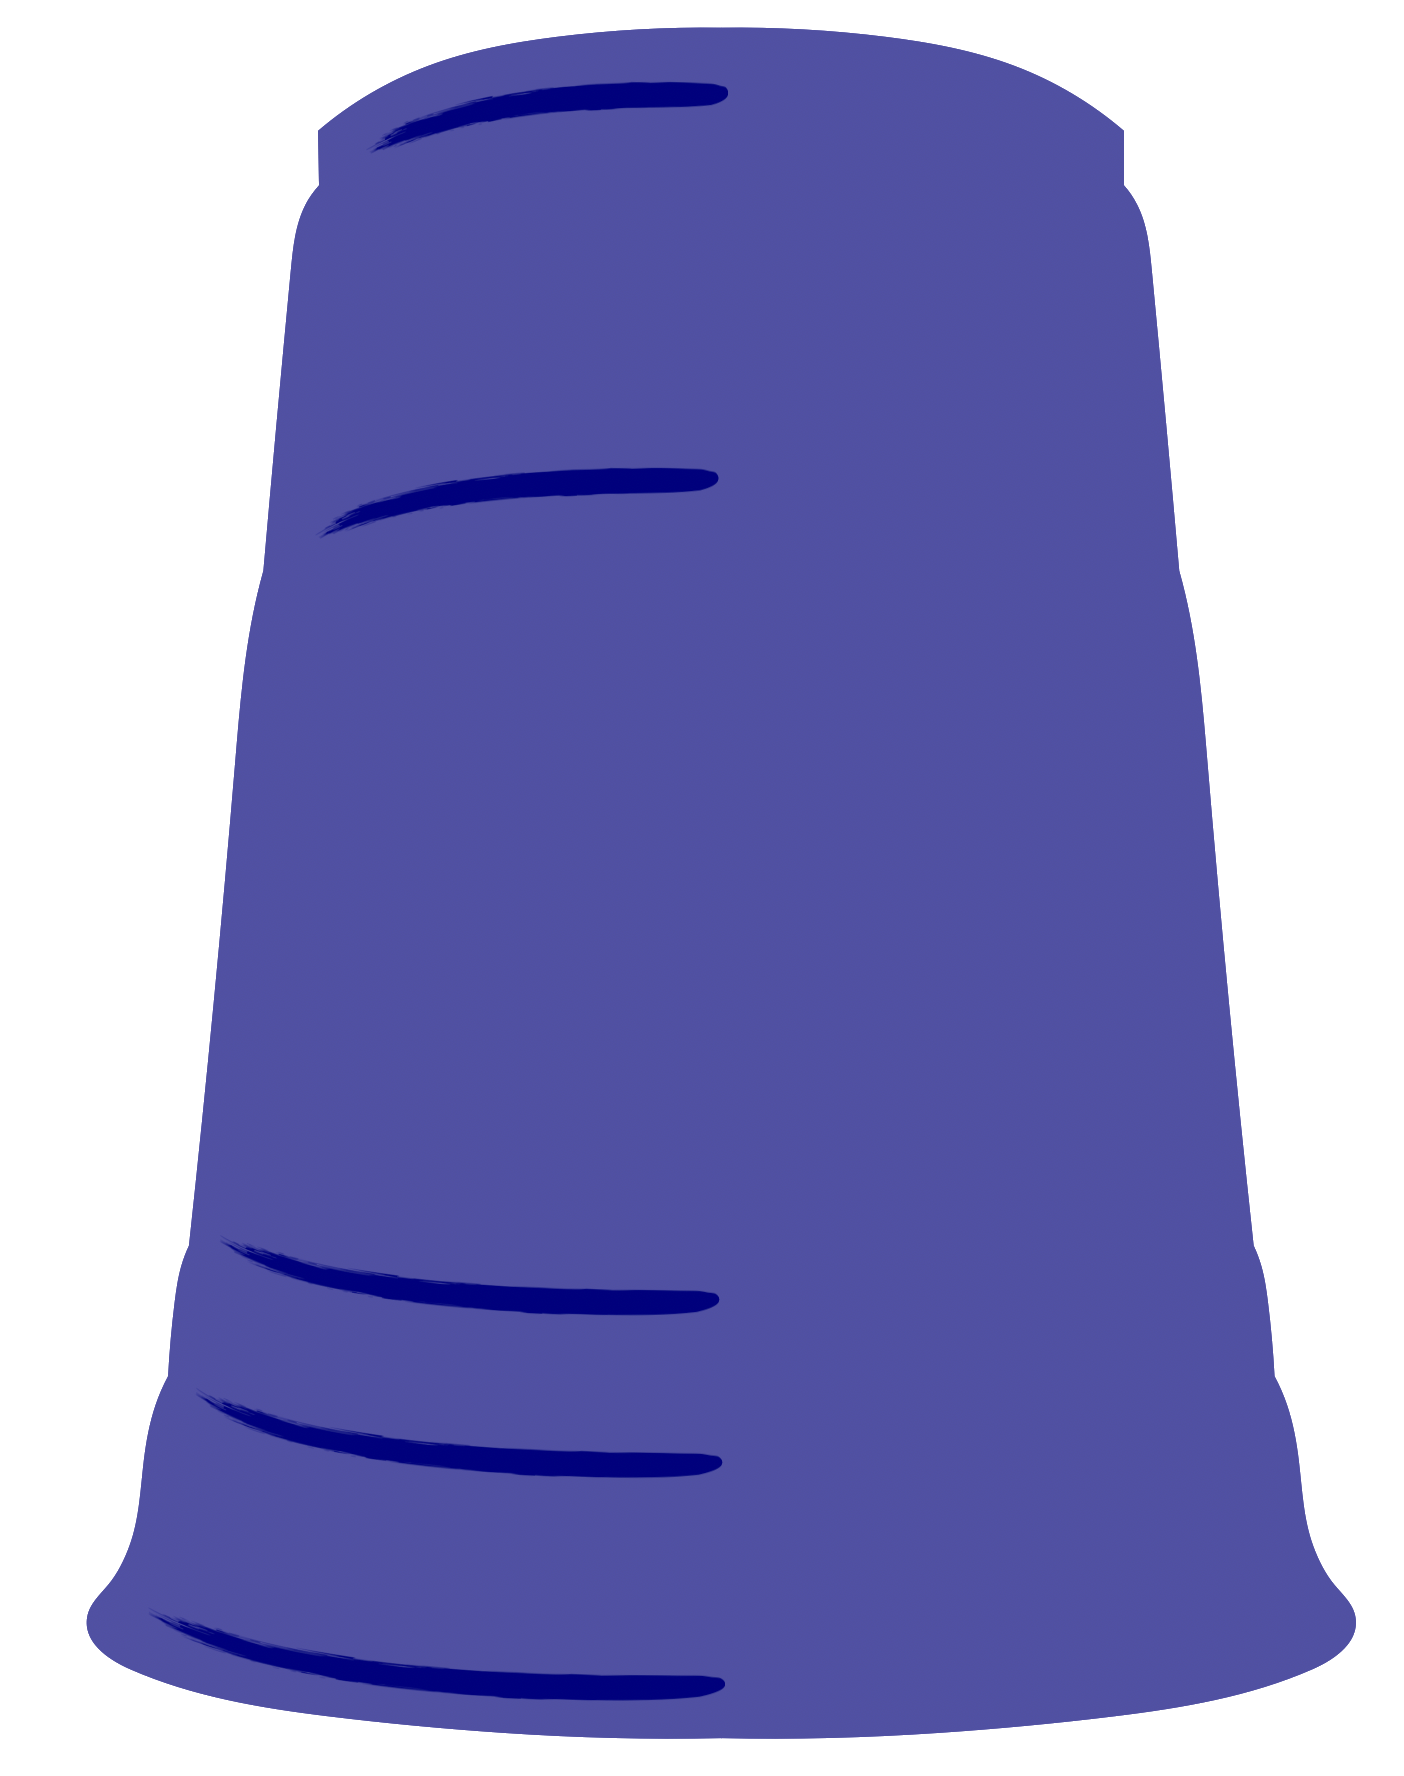
\includegraphics[width=2cm]{cup_down.png}};
        \begin{scope}[scale=0.7, shift={(-17, 3)}, rotate=-5]
            \fill[dark, rounded corners=3] (0, 0) rectangle (10, 6);
            \fill[black] (0, 0.5) rectangle (10, 3.5);
            \node[text=white, align=center, rotate=-5] at (5, 5.2) { \small \textsf{OLÁ} };
            \node[text=white, align=center, rotate=-5] at (5, 4.1) { \tiny \textsf{meu nome é } };
            \node[text=white, align=center, rotate=0] at (5.25, 2) { \large \textsl{Grupo 1} };
          \end{scope}

        \fill[dark] (0, 4) circle (1);
        \node at (0, 7) {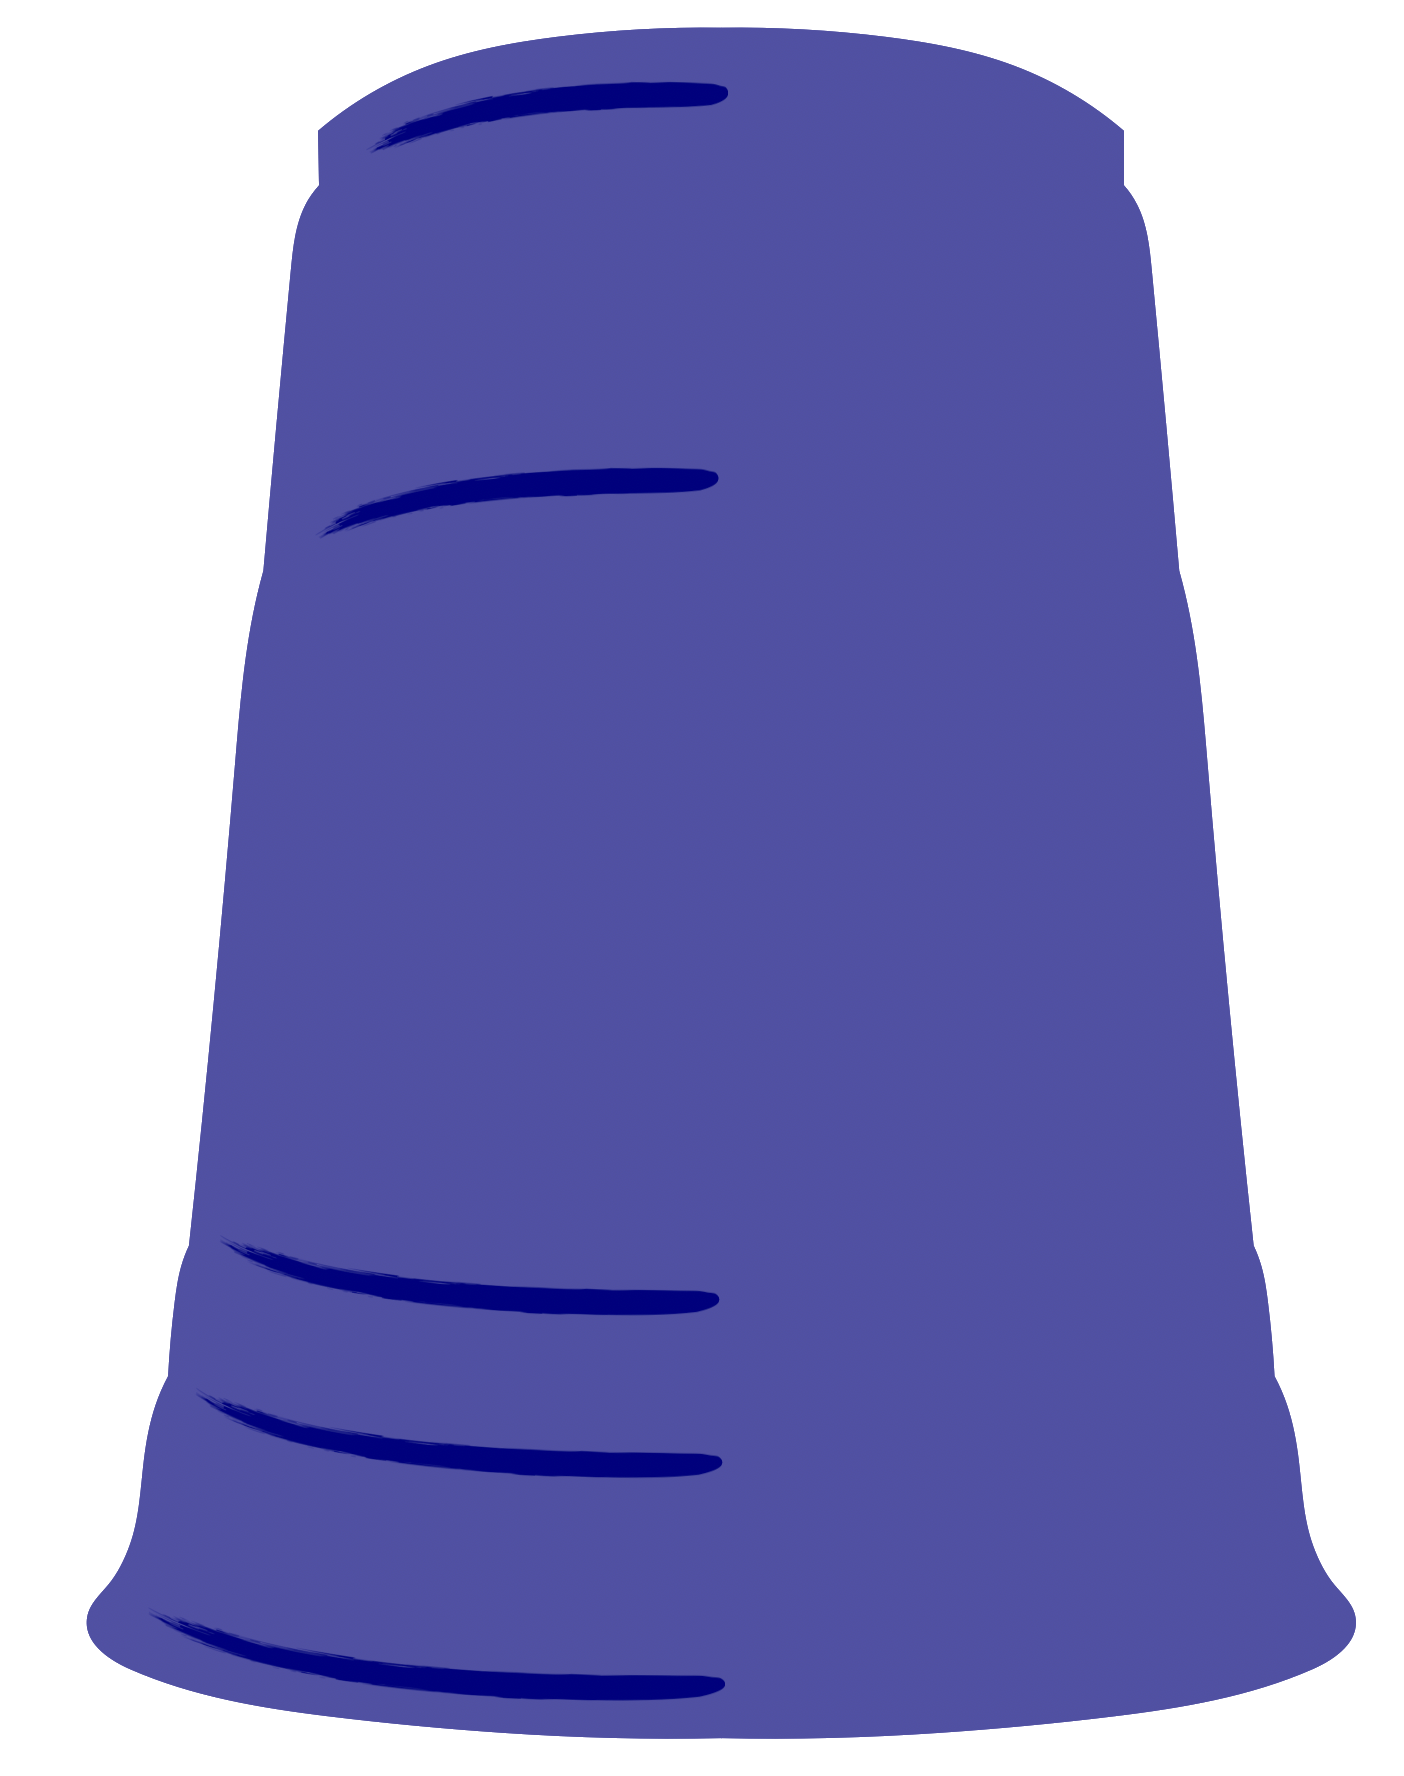
\includegraphics[width=2cm]{cup_down.png}};
        \begin{scope}[scale=0.7, shift={(-2, 3)}, rotate=10]
            \fill[dark, rounded corners=3] (0, 0) rectangle (10, 6);
            \fill[black] (0, 0.5) rectangle (10, 3.5);
            \node[text=white, align=center, rotate=10] at (5, 5.2) { \small \textsf{OLÁ} };
            \node[text=white, align=center, rotate=10] at (5, 4.1) { \tiny \textsf{meu nome é } };
            \node[text=white, align=center, rotate=7] at (5.25, 2) { \large \textsl{Grupo 2} };
          \end{scope}

        \fill[dark] (+10, 4) circle (1);
        \node at (+10, 7) {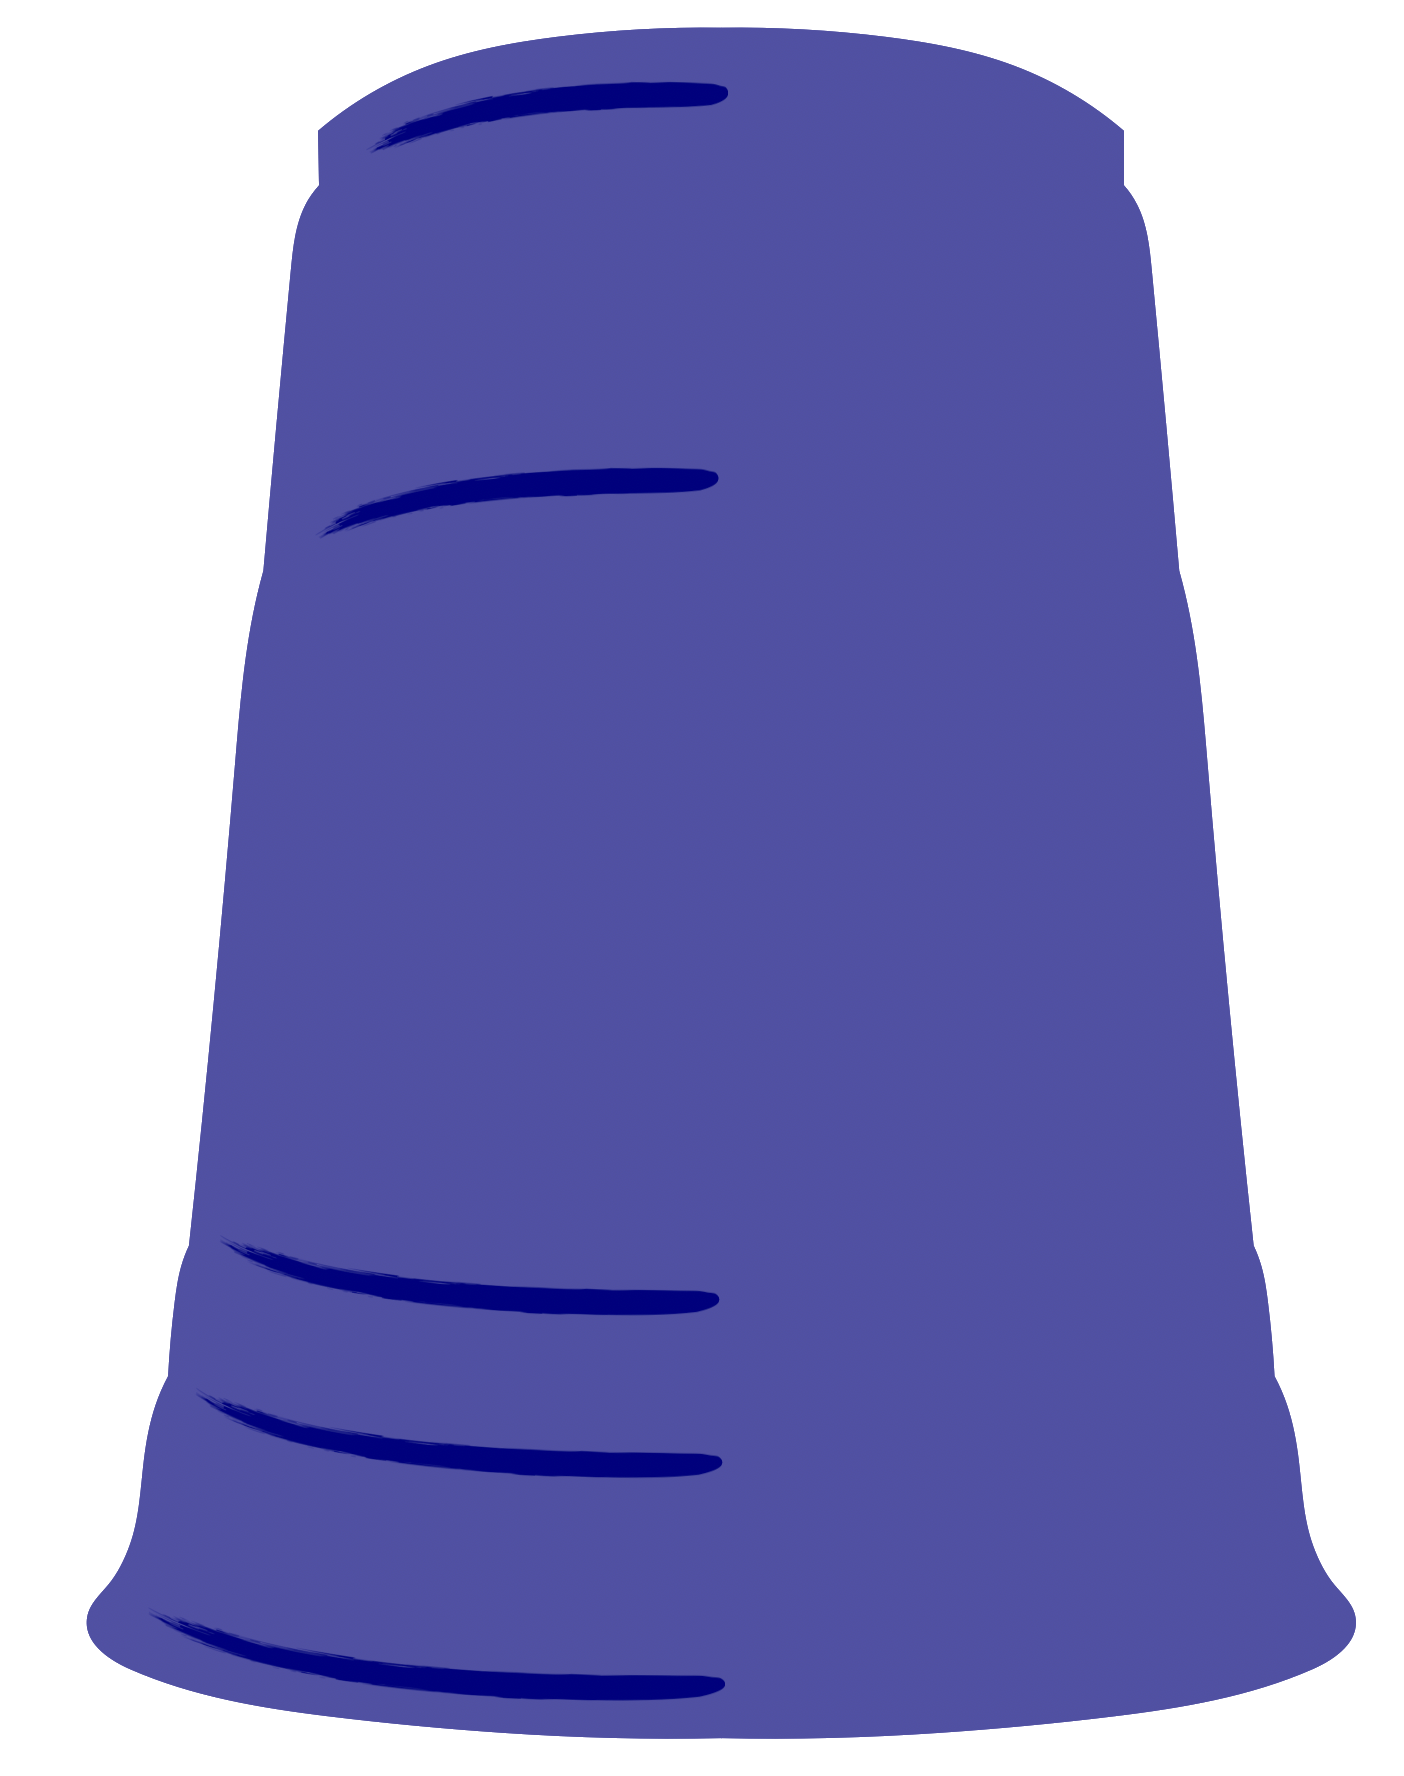
\includegraphics[width=2cm]{cup_down.png}};
        \begin{scope}[scale=0.7, shift={(12, 3)}, rotate=1]
            \fill[dark, rounded corners=3] (0, 0) rectangle (10, 6);
            \fill[black] (0, 0.5) rectangle (10, 3.5);
            \node[text=white, align=center, rotate=1] at (5, 5.2) { \small \textsf{OLÁ} };
            \node[text=white, align=center, rotate=1] at (5, 4.1) { \tiny \textsf{meu nome é } };
            \node[text=white, align=center, rotate=1] at (5.25, 2) { \large \textsl{Grupo 3} };
          \end{scope}
        \end{scope}
        \end{tikzpicture}
    \end{adjustbox}
\end{frame}

\begin{frame}{Revisitando a Permutabilidade \parencite{definettiTheoryProbability1974}\footnote{figuras adaptadas de \href{https://betanalpha.github.io/assets/case_studies/hierarchical_modeling.html}{Michael Betancourt (CC-BY-SA-4.0)}}}
    \begin{adjustbox}{max width=1.0\textwidth}
        \begin{tikzpicture}[scale=0.3, thick]


            \draw[white] (-17, -3) rectangle (17, 15);

            \fill[dark] (-10, 4) circle (1);
            \node at (-10, 7) {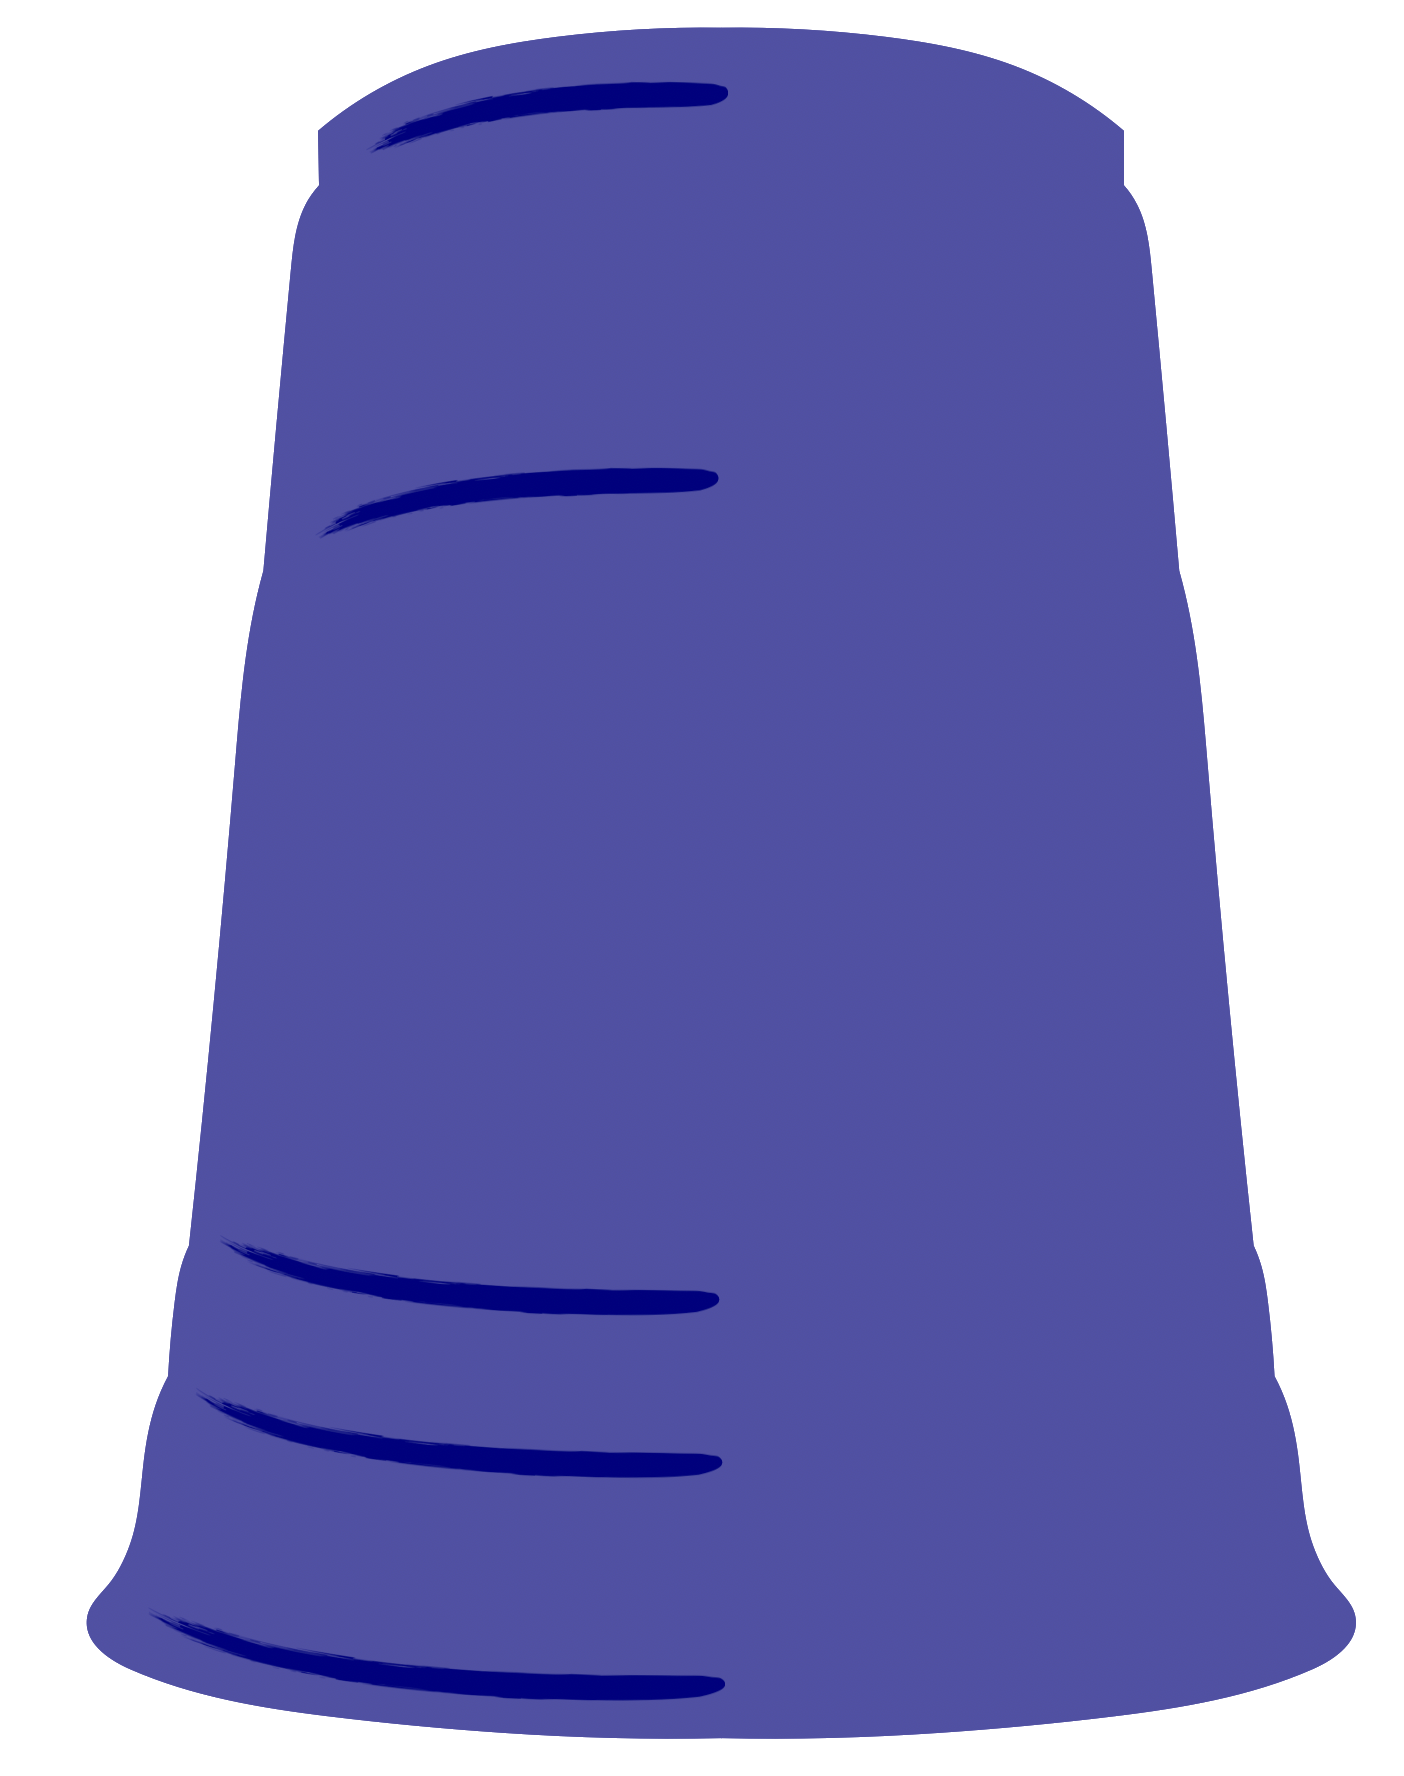
\includegraphics[width=2cm]{cup_down.png}};

            % Left
            \begin{scope}[scale=0.7, shift={(-17, 3)}, rotate=-5]
              \fill[dark, rounded corners=3] (0, 0) rectangle (10, 6);
              \fill[black] (0, 0.5) rectangle (10, 3.5);
              \node[text=white, align=center, rotate=-5] at (5, 5.2) { \small \textsf{OLÁ} };
              \node[text=white, align=center, rotate=-5] at (5, 4.1) { \tiny \textsf{meu nome é } };
              \node[text=white, align=center, rotate=0] at (5.25, 2) { \large \textsl{Grupo 1} };
            \end{scope}

            \fill[dark] (0, 4) circle (1);
            \node at (0, 7) {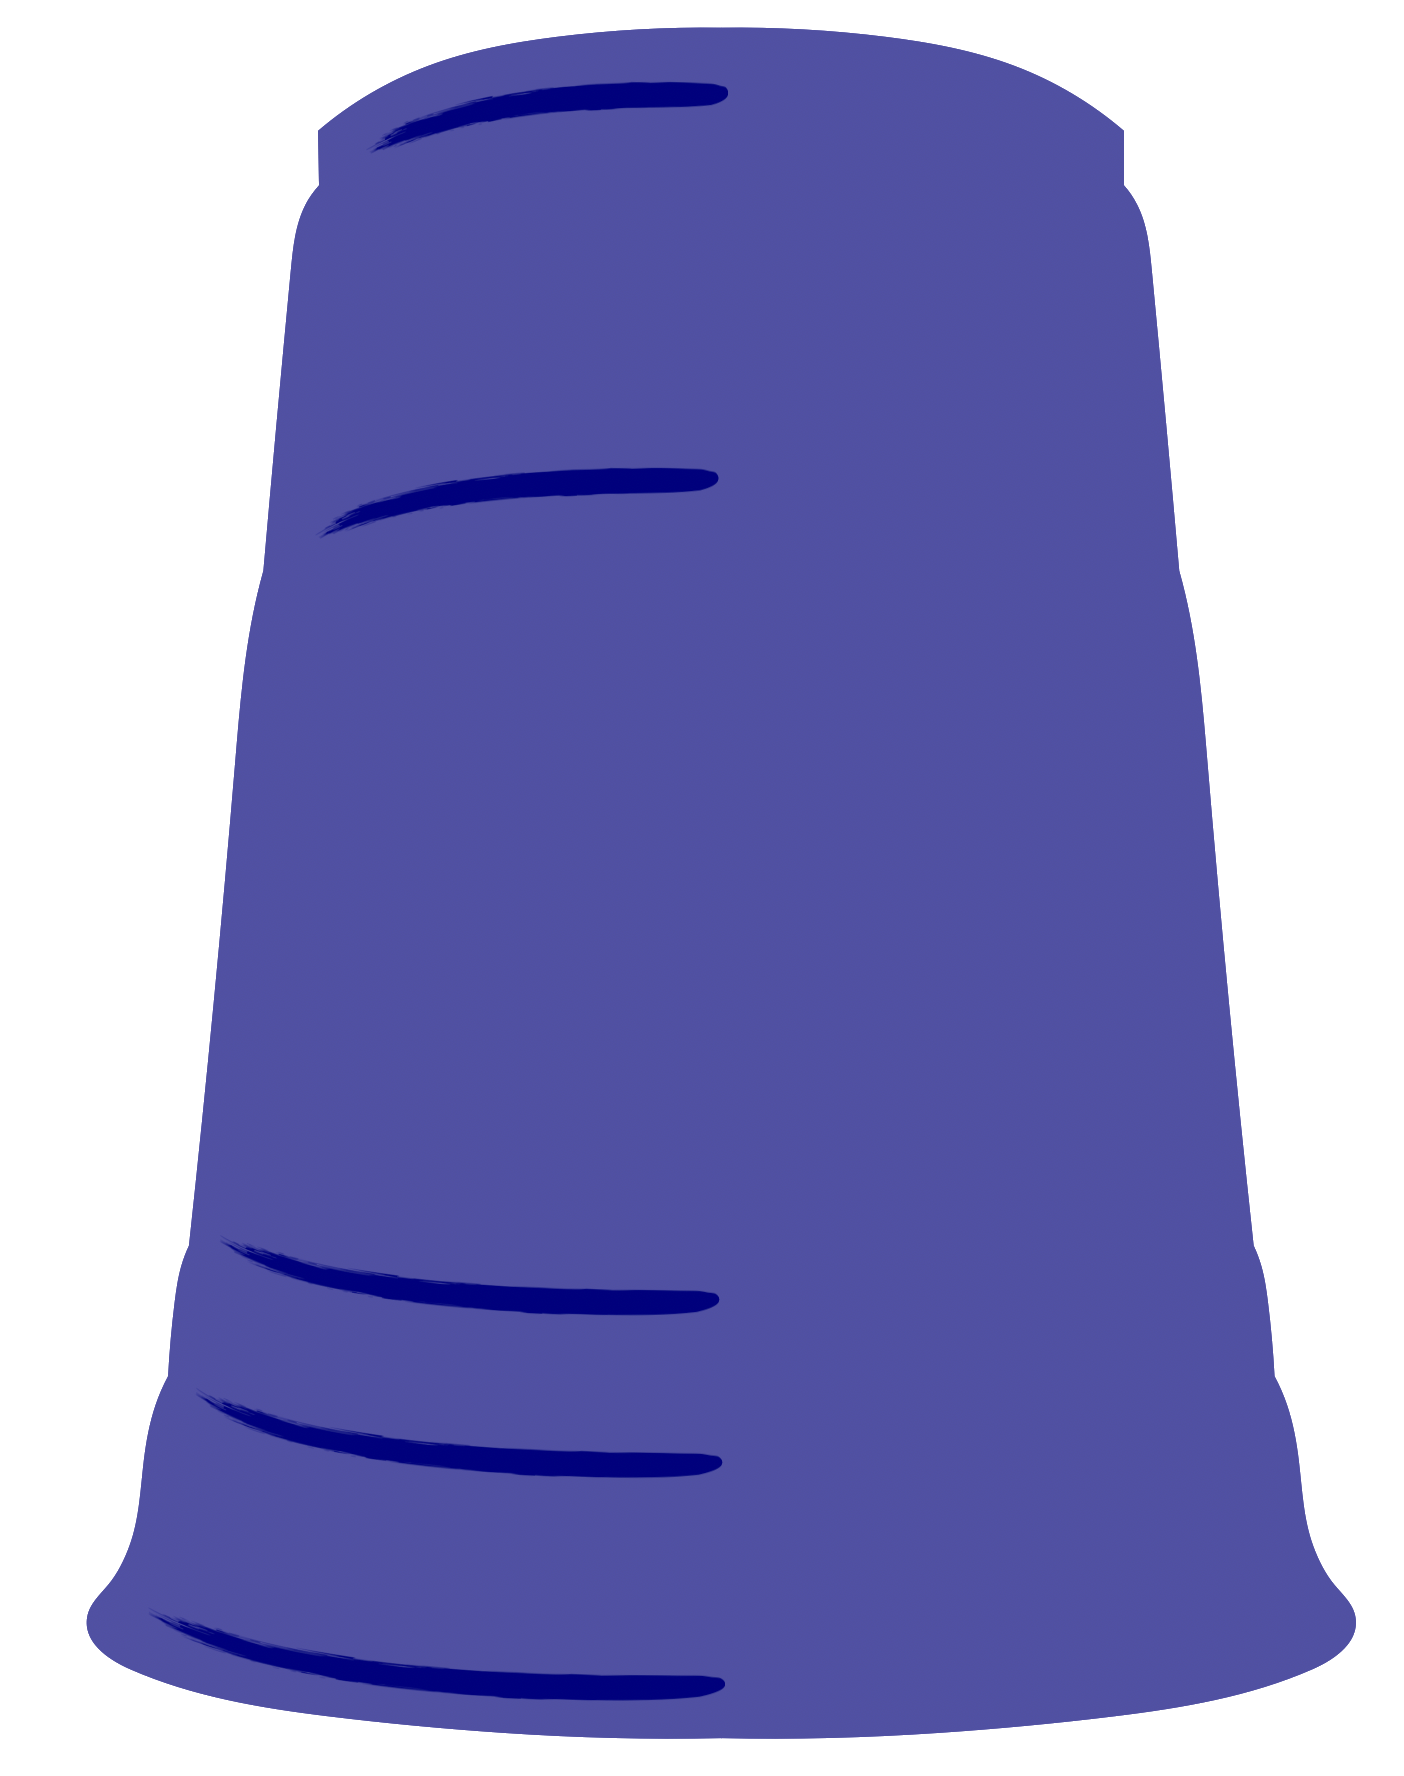
\includegraphics[width=2cm]{cup_down.png}};

            \begin{scope}[scale=0.7, shift={(-2, 3)}, rotate=10]
              \fill[dark, rounded corners=3] (0, 0) rectangle (10, 6);
              \fill[black] (0, 0.5) rectangle (10, 3.5);
              \node[text=white, align=center, rotate=10] at (5, 5.2) { \small \textsf{OLÁ} };
              \node[text=white, align=center, rotate=10] at (5, 4.1) { \tiny \textsf{meu nome é } };
              \node[text=white, align=center, rotate=7] at (5.25, 2) { \large \textsl{Grupo 2} };
            \end{scope}

            \fill[dark] (+10, 4) circle (1);
            \node at (+10, 7) {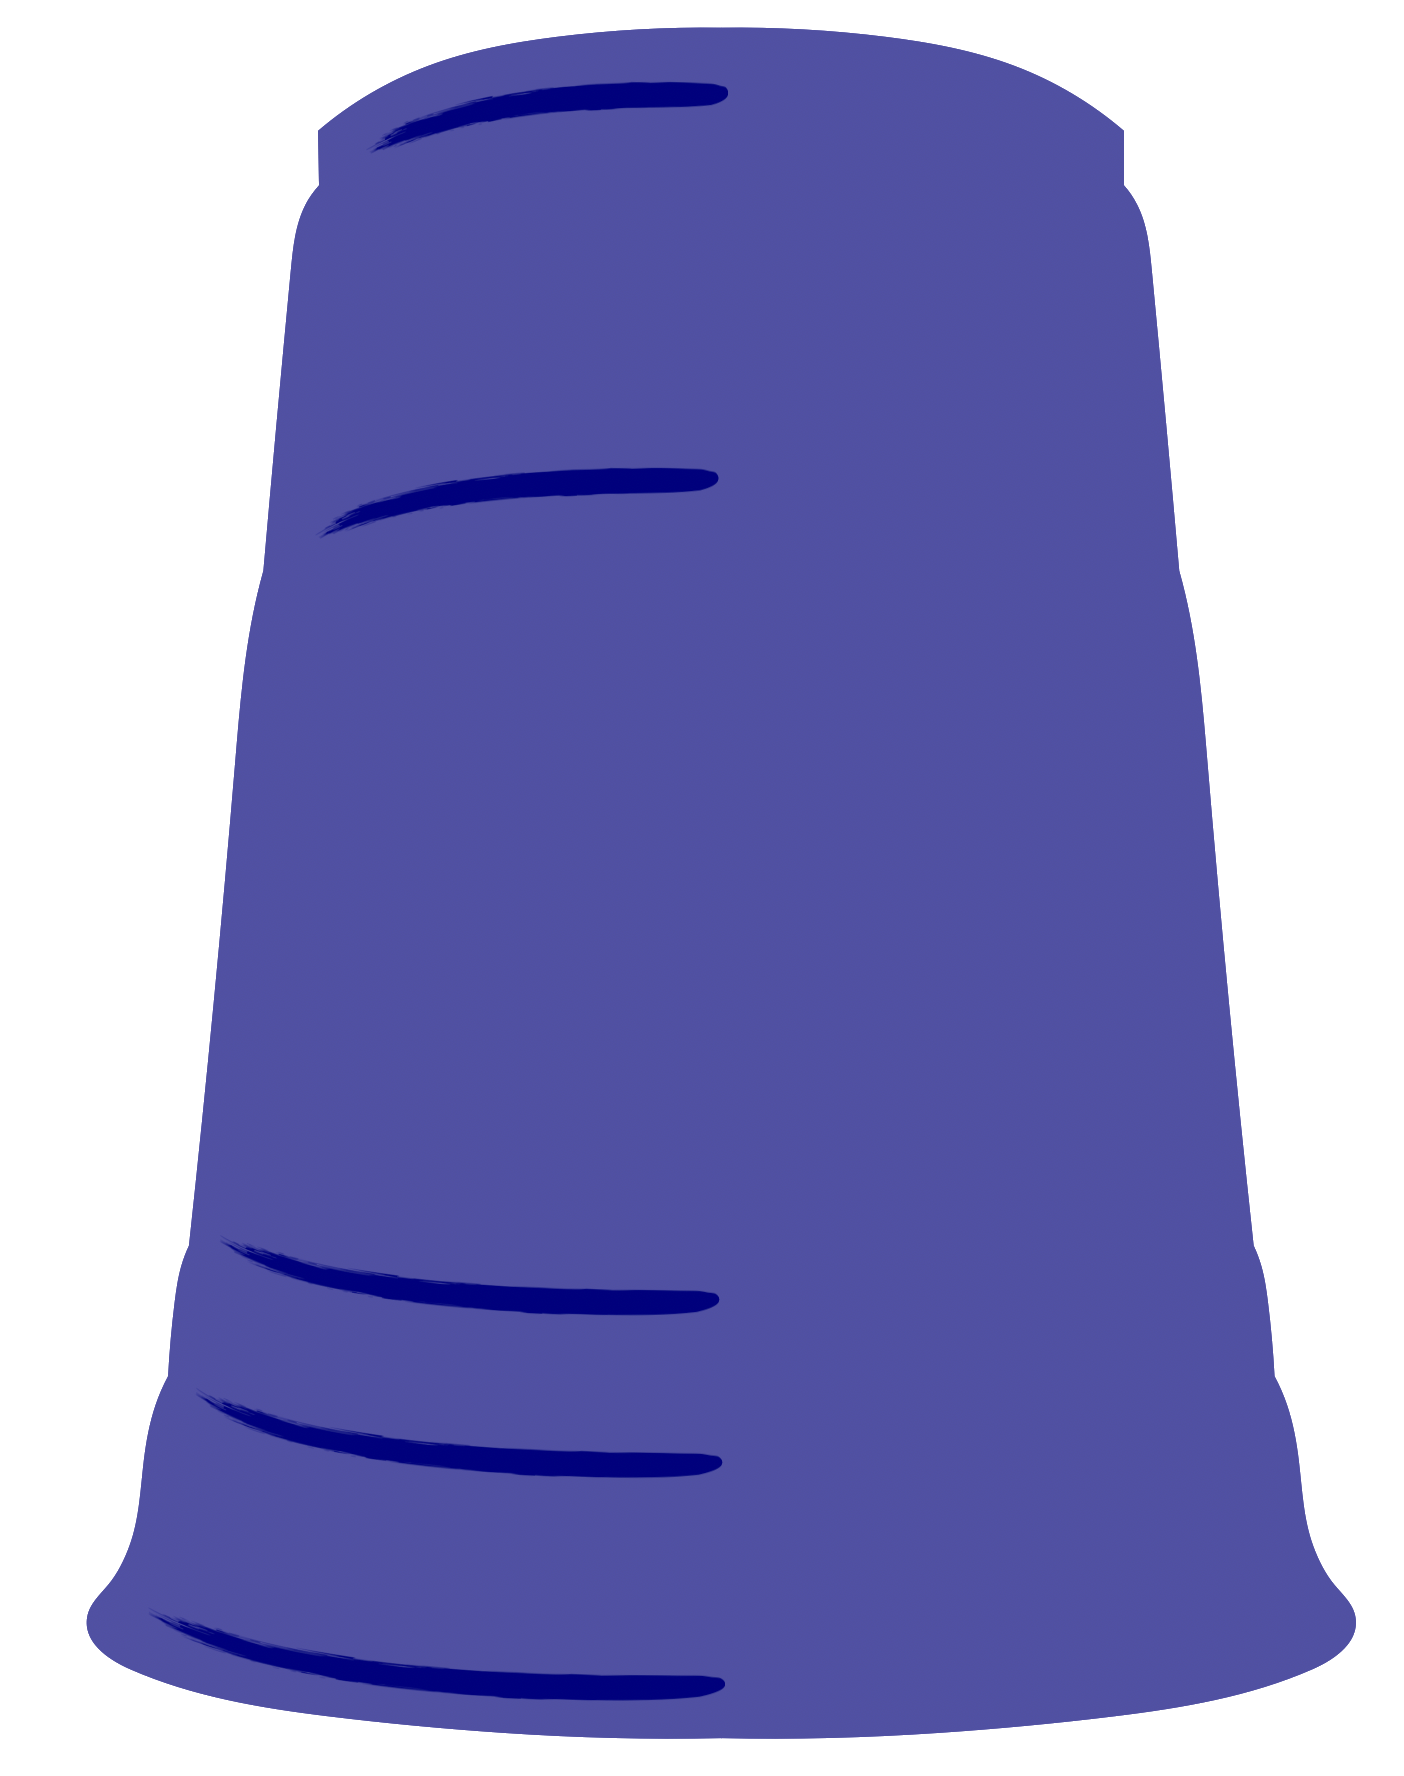
\includegraphics[width=2cm]{cup_down.png}};

            \begin{scope}[scale=0.7, shift={(12, 3)}, rotate=1]
              \fill[dark, rounded corners=3] (0, 0) rectangle (10, 6);
              \fill[black] (0, 0.5) rectangle (10, 3.5);
              \node[text=white, align=center, rotate=1] at (5, 5.2) { \small \textsf{OLÁ} };
              \node[text=white, align=center, rotate=1] at (5, 4.1) { \tiny \textsf{meu nome é } };
              \node[text=white, align=center, rotate=1] at (5.25, 2) { \large \textsl{Grupo 3} };
            \end{scope}

            \pgfmathsetmacro{\r}{10}
            \pgfmathsetmacro{\start}{160}
            \pgfmathsetmacro{\stop}{20}

            \draw[dark, <->, >=stealth] ({0 + \r * cos(\start)}, {8 + \r * sin(\start)})
                            arc[x radius = \r, y radius = 3, start angle=\start, end angle= \stop];

            \pgfmathsetmacro{\r}{3}
            \pgfmathsetmacro{\start}{160}
            \pgfmathsetmacro{\stop}{20}

            \draw[dark, <->, >=stealth] ({-5 + \r * cos(\start)}, {10 + \r * sin(\start)})
                            arc[x radius = \r, y radius = 0.75, start angle=\start, end angle= \stop];

            \draw[dark, <->, >=stealth] ({5 + \r * cos(\start)}, {10 + \r * sin(\start)})
                            arc[x radius = \r, y radius = 0.75, start angle=\start, end angle= \stop];

            % Right
            \begin{scope}[shift={(36, 0)}]

            \draw[white] (-17, -3) rectangle (17, 15);

            \fill[dark] (-10, 4) circle (1);
            \node at (-10, 7) {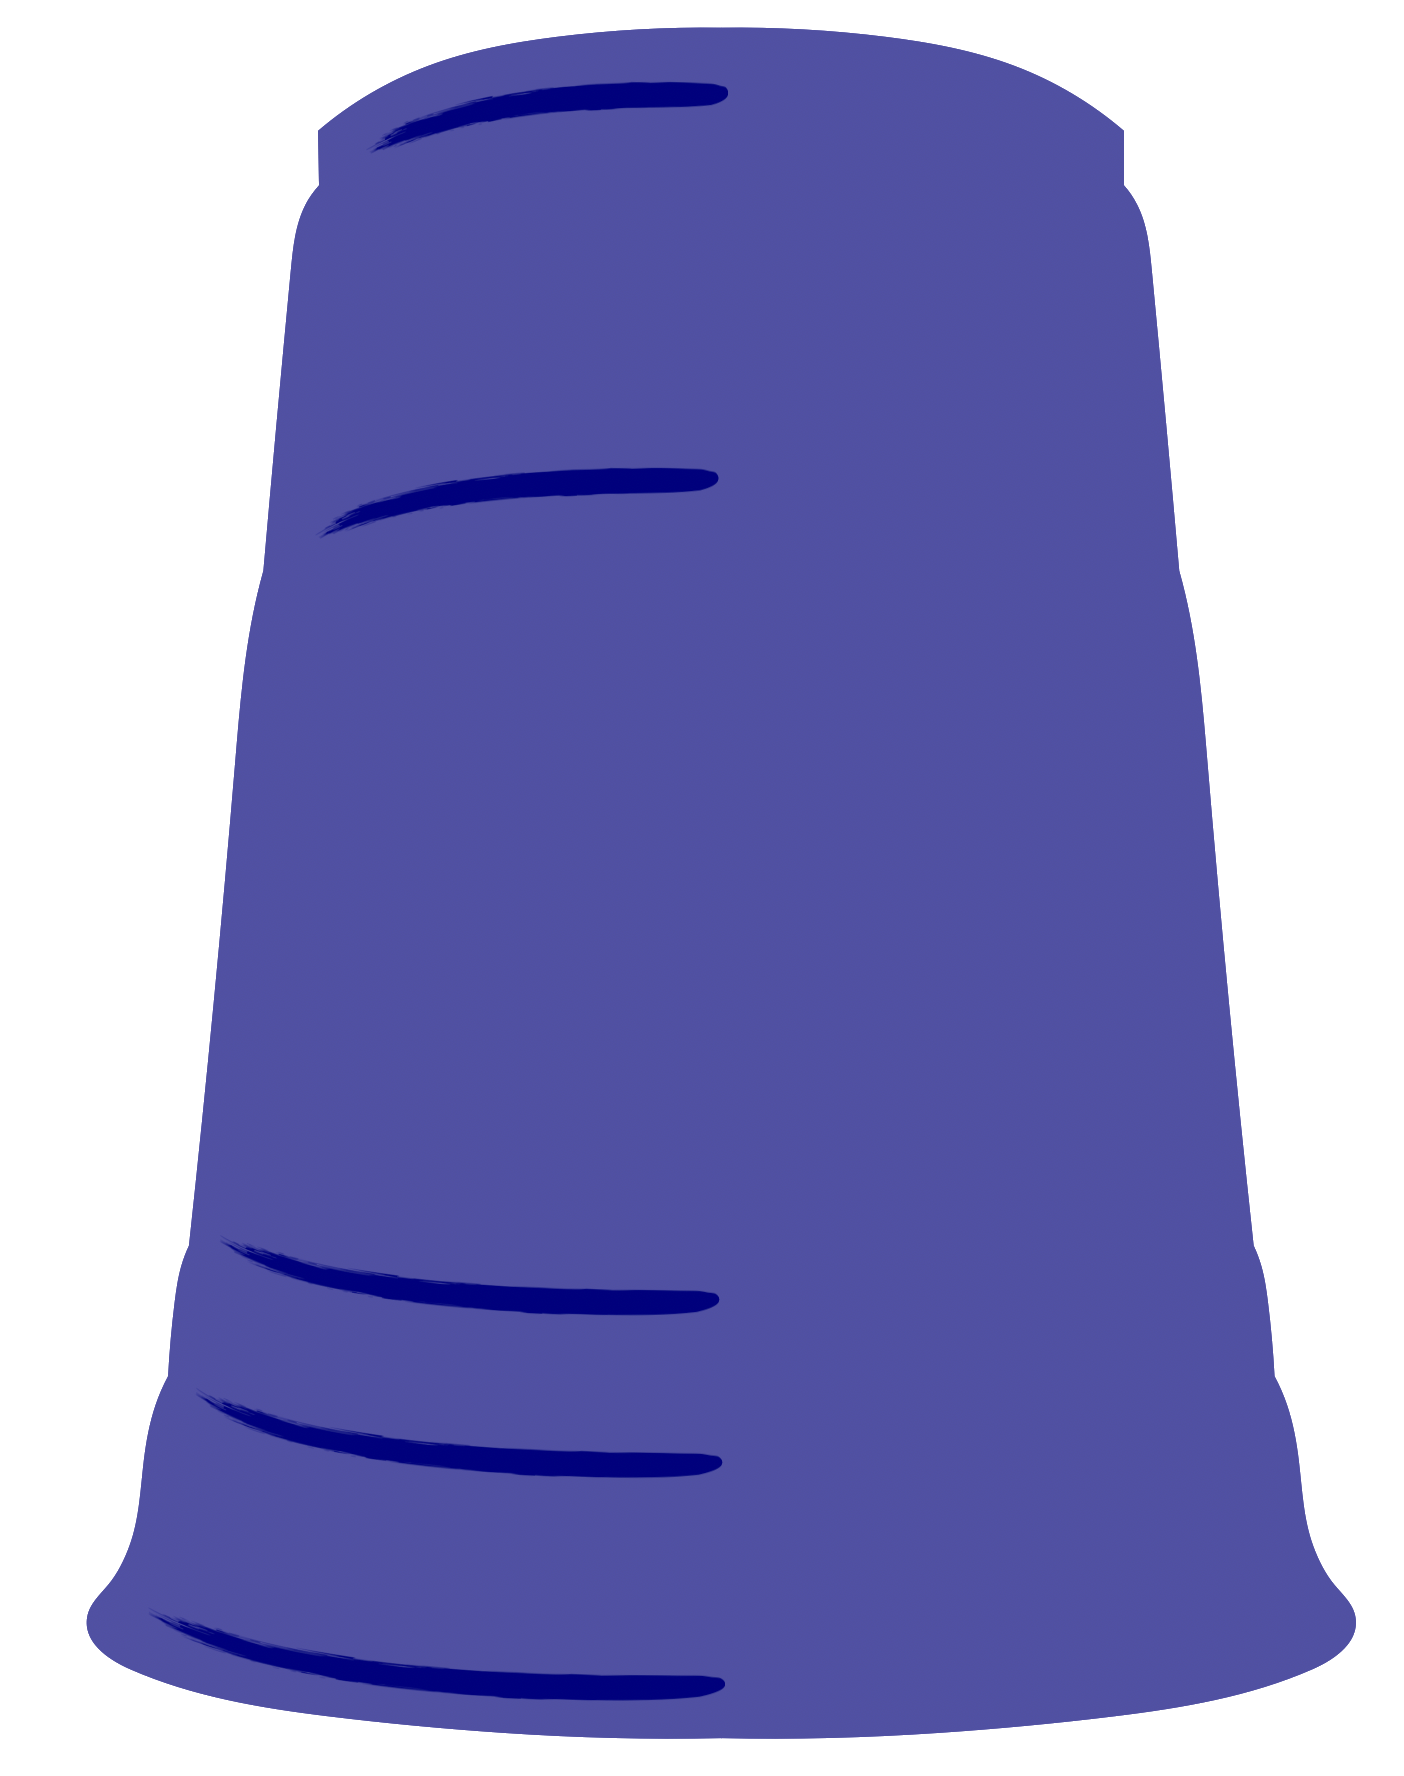
\includegraphics[width=2cm]{cup_down.png}};

            \begin{scope}[scale=0.7, shift={(-17, 3)}, rotate=-5]
              \fill[dark, rounded corners=3] (0, 0) rectangle (10, 6);
              \fill[black] (0, 0.5) rectangle (10, 3.5);
              \node[text=white, align=center, rotate=-5] at (5, 5.2) { \small \textsf{OLÁ} };
              \node[text=white, align=center, rotate=-5] at (5, 4.1) { \tiny \textsf{meu nome é } };
              \node[text=white, align=center, rotate=0] at (5.25, 2) { \large \textsl{Grupo 3} };
            \end{scope}

            \fill[dark] (0, 4) circle (1);
            \node at (0, 7) {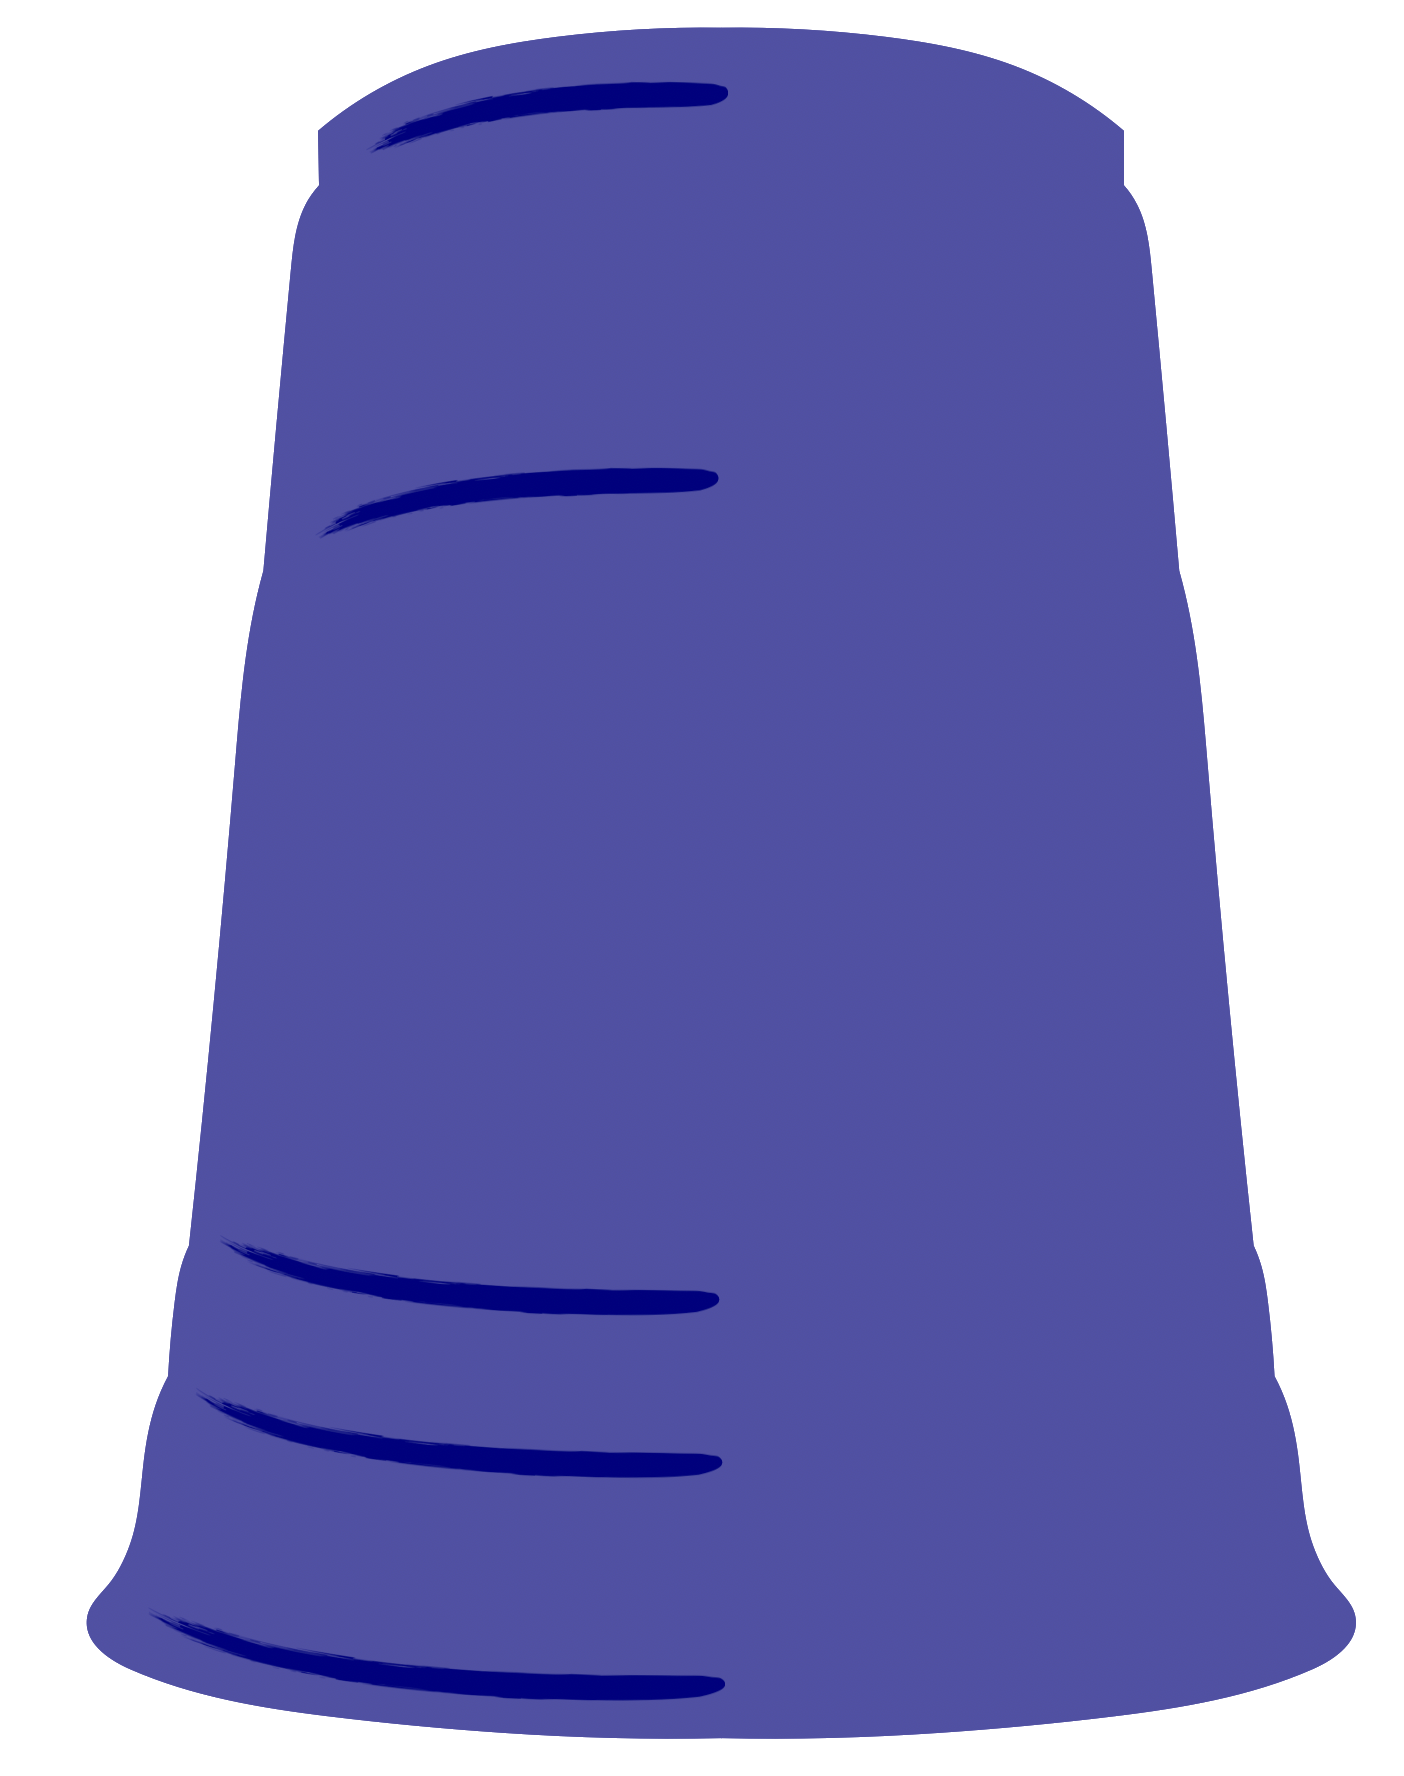
\includegraphics[width=2cm]{cup_down.png}};

            \begin{scope}[scale=0.7, shift={(-2, 3)}, rotate=10]
              \fill[dark, rounded corners=3] (0, 0) rectangle (10, 6);
              \fill[black] (0, 0.5) rectangle (10, 3.5);
              \node[text=white, align=center, rotate=10] at (5, 5.2) { \small \textsf{OLÁ} };
              \node[text=white, align=center, rotate=10] at (5, 4.1) { \tiny \textsf{meu nome é } };
              \node[text=white, align=center, rotate=7] at (5.25, 2) { \large \textsl{Grupo 1} };
            \end{scope}

            \fill[dark] (+10, 4) circle (1);
            \node at (+10, 7) {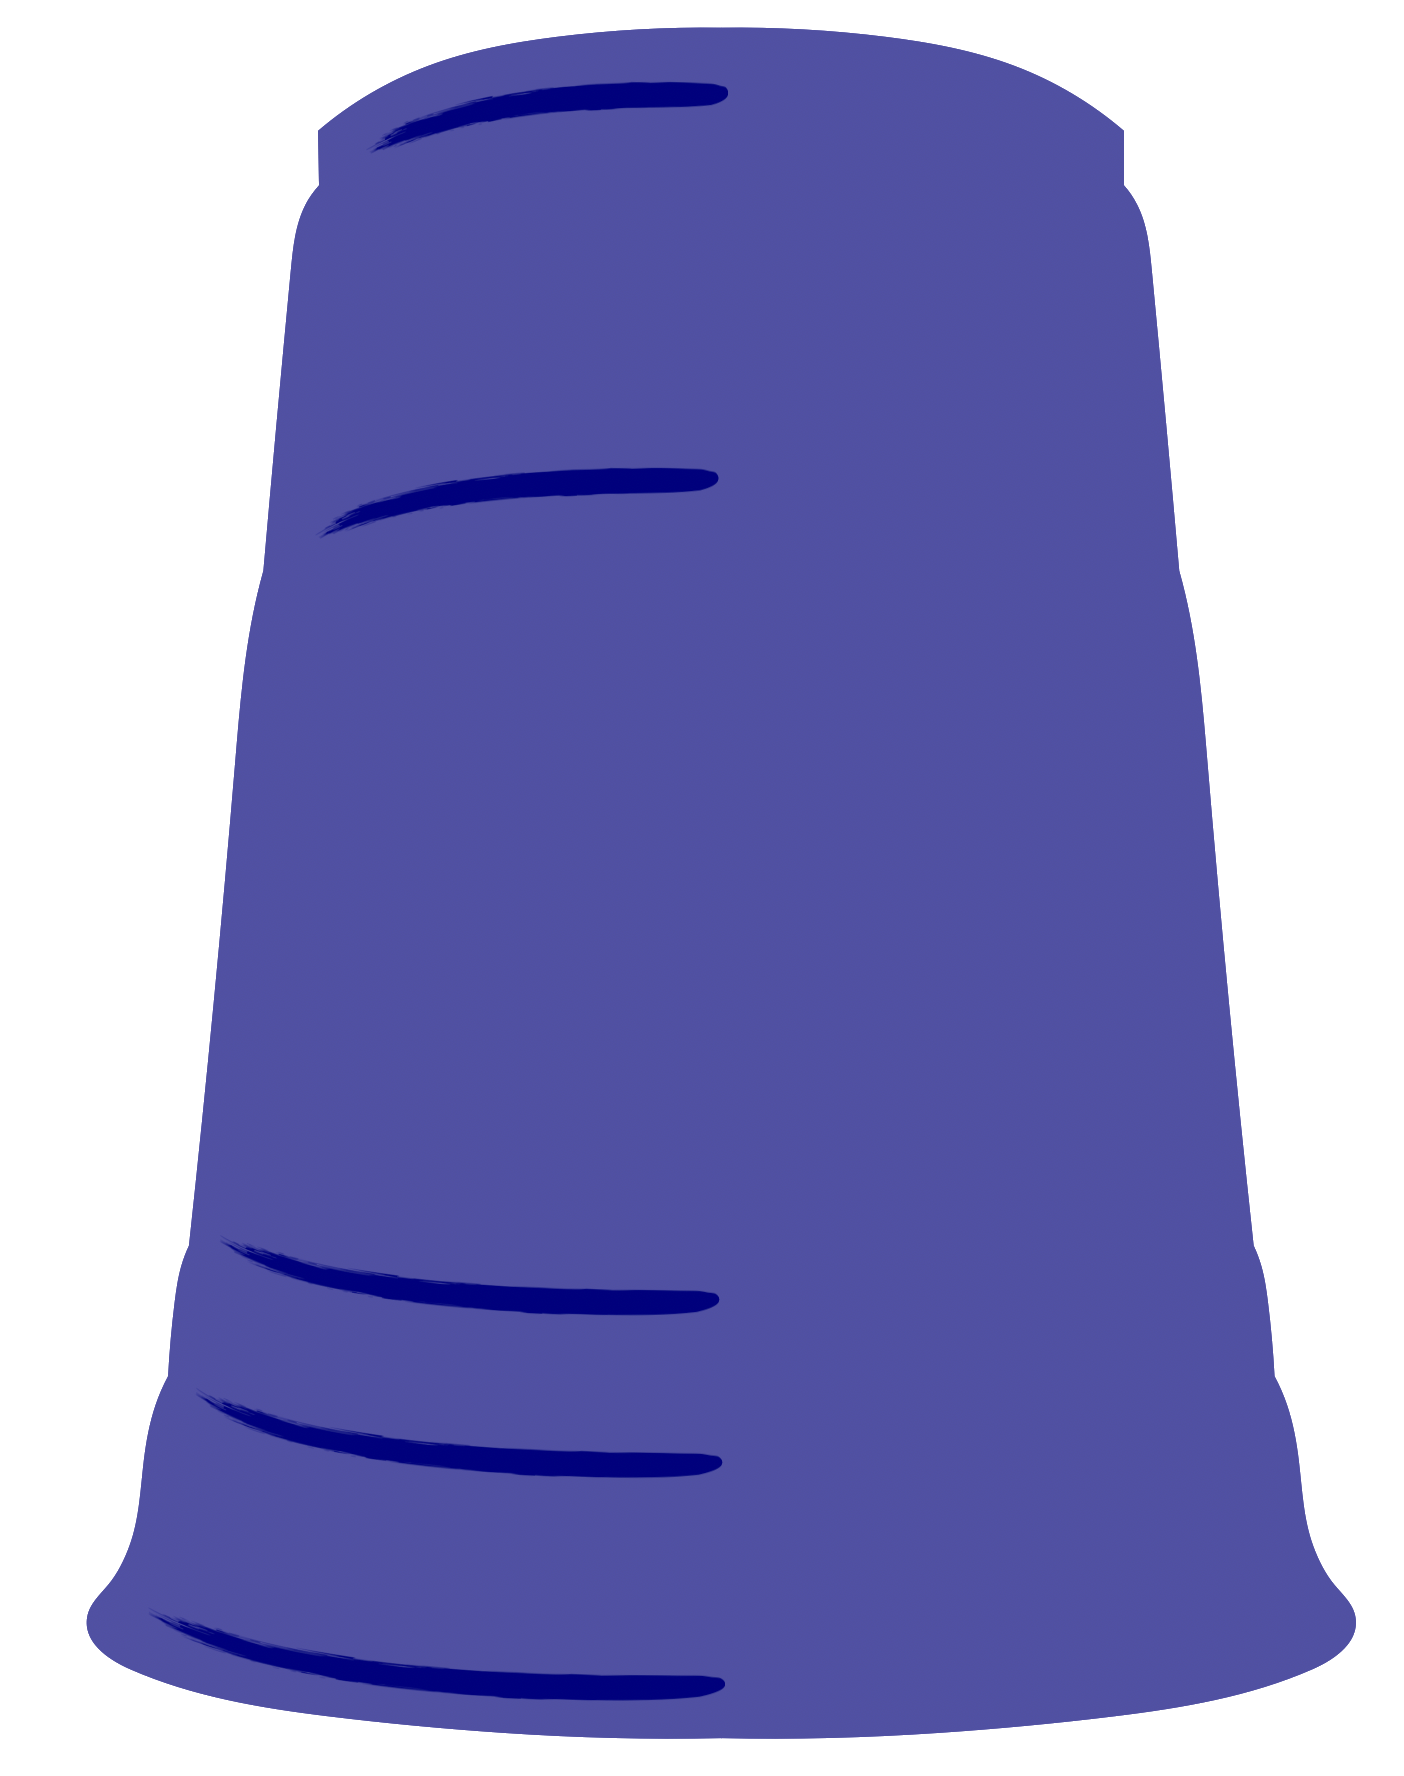
\includegraphics[width=2cm]{cup_down.png}};

            \begin{scope}[scale=0.7, shift={(12, 3)}, rotate=1]
              \fill[dark, rounded corners=3] (0, 0) rectangle (10, 6);
              \fill[black] (0, 0.5) rectangle (10, 3.5);
              \node[text=white, align=center, rotate=1] at (5, 5.2) { \small \textsf{OLÁ} };
              \node[text=white, align=center, rotate=1] at (5, 4.1) { \tiny \textsf{meu nome é } };
              \node[text=white, align=center, rotate=1] at (5.25, 2) { \large \textsl{Grupo 2} };
            \end{scope}

            \draw[light, <->, >=stealth, line width=4]
              (-8, 6.5) .. controls (-7, 7.5) and (-6.5, 8.25) ..
              (-4.5, 8.5) .. controls (-2.5, 8.75) and (-1, 8.5) .. (0, 7);
            \draw[dark, <->, >=stealth, line width=2]
              (-7.85, 6.65) .. controls (-7, 7.5) and (-6.5, 8.25) ..
              (-4.5, 8.5) .. controls (-2.5, 8.75) and (-1, 8.5) .. (-0.15, 7.15);

            \draw[light, <->, >=stealth, line width=4]
              (3, 7.5) .. controls (4, 9) and (6.25, 9.75) ..
              (8.25, 9.5) .. controls (10.25, 9.25) and (11, 8.75) .. (12, 6.75);
            \draw[dark, <->, >=stealth, line width=2]
              (3.15, 7.65) .. controls (4, 9) and (6.25, 9.75) ..
              (8.25, 9.5) .. controls (10.25, 9.25) and (11, 8.75) .. (11.9, 6.9);

            \draw[light, <->, >=stealth, line width=4]
              (-8, 1.5) .. controls (-7, -1.5) and (2, -1.25) ..
              (4, -1) .. controls (6, -0.75) and (11, -0.5) .. (12, 1.5);
            \draw[dark, <->, >=stealth, line width=2]
              (-7.925, 1.25) .. controls (-7, -1.5) and (2, -1.25) ..
              (4, -1) .. controls (6, -0.75) and (11, -0.5) .. (11.9, 1.3);

            \end{scope}

            \end{tikzpicture}
    \end{adjustbox}
\end{frame}

\subsection{\textit{Hiperpriori} (\textit{Hyperprior})}
\begin{frame}{\textit{Hiperpriori} (\textit{Hyperprior})}
    Em modelos multiníveis temos a figura da \textit{hiperpriori}, que é
    justamente uma \textit{priori} de uma \textit{priori}:
    $$
    \begin{aligned}
        \boldsymbol{y} &\sim \text{Normal}(10, \boldsymbol{\theta}) \\
        \boldsymbol{\theta} &\sim \text{Normal}(0, \phi) \\
        \phi &\sim \text{Exponencial(1)}
    \end{aligned}
    $$
    Aqui $\boldsymbol{y}$ são variáveis de interesse que pertencem à certos
    grupos distintos. $\boldsymbol{\theta}$, uma \textit{priori} de $\boldsymbol{y}$,
    é um vetor de parâmetros de grupos com uma \textit{priori} (que se torna \textit{hyperiori})
    $\phi$.
\end{frame}

\subsection{Abordagem Frequentista versus Abordagem Bayesiana}
\begin{frame}{Abordagem Frequentista versus Abordagem Bayesiana}
  Existem modelos multíveis também na estatística frequentista.
  Todos esses estão disponíveis no pacote \texttt{lme4} \parencite{lme4}.
  \begin{vfilleditems}
    \item \textbf{otimização da função de verossimilhança} versus \textbf{aproximação da posterior via MCMC}.
    Quase sempre isso gera falha de convergência para modelos que não sejam extremamente
    simples.
    \item \textbf{modelos multiníveis frequentista não computam $p$-valores dos efeitos de grupo}\footnote{veja a explicação \href{https://stat.ethz.ch/pipermail/r-help/2006-May/094765.html}{aqui do Douglas Bates autor do pacote \texttt{lme4}}}.
    or conta da contorção matemática de diversas aproximações que a estatística
    frequentista tem que fazer o cálculo de $p$-valores de efeitos de
    grupo possuem fortes pressupostos. O principal é que os grupos são balanceados.
    Ou seja, os grupos são homogêneos no seu tamanho.
    Qualquer desbalanço na composição dos grupos (um grupo com mais observações que outros) resulta em
    $p$-valores patológicos e que não podem ser confiáveis.
  \end{vfilleditems}
\end{frame}

\begin{frame}{Abordagem Frequentista versus Abordagem Bayesiana}
  Sumarizando, a abordagem \textbf{frequentista para modelos multiníveis não é robusta}
  tanto no processo da \textbf{inferência} (\textbf{falhas de convergência}
  da estimação de máxima verossimilhança), quanto nos \textbf{resultados} dessa
  inferência (não computa $p$-valores por conta de \textbf{fortes pressupostos
  que quase sempre são violados}).
\end{frame}

\subsection{3 Abordagens de Modelos Multiníveis}

\begin{frame}{3 Abordagens de Modelos Multiníveis}
  \begin{vfilleditems}
    \item \textit{Random-intercept model}: Modelo no qual cada grupo recebe uma
    constante (\textit{intercept}) diferente além da constante global e coeficientes
    globais
    \item \textit{Random-slope model}: Modelo no qual cada grupo recebe um coeficiente
    (\textit{slope}) diferente para cada variável independente além da constante global
    \item \textit{Random-intercept-slope model}: Modelo no qual cada grupo recebe tanto
    uma constante (\textit{intercept}) quanto um coeficiente (\textit{slope})
    diferente para cada variável independente além da constante global
  \end{vfilleditems}
  \small
  \texttt{rstanarm} e \texttt{brms} possuem as funcionalidades completas para rodar
  modelos multiníveis e a única coisa a se fazer é alterar a fórmula. Para
  \texttt{rstanarm}, há uma segunda mudança também que não usamos mais a função
  \texttt{stan\_glm()} mas sim a função \texttt{stan\_glmer()}. Para \texttt{brms}
  não há mudança e usamos a mesma função \texttt{brm()}.
\end{frame}

\subsubsection{\textit{Random-intercept model}}
\begin{frame}[fragile]{\textit{Random-intercept model}}
  A primeira abordagem é o \textit{random-intercept model} na qual especificamos
  para cada grupo uma constante diferente, além da constante global. Essas constantes
  são amostradas de uma \textit{hiperpriori}.
  \vfill
  A fórmula a ser usada segue este padrão:
  \begin{lstlisting}
    y ~ (1 | group) + x1 + x2
  \end{lstlisting}
  \vfill
  O \texttt{(1 | group)} na fórmula sinaliza que a constante \texttt{1}
  deve ser também especificada para cada um dos grupos listados nos valores
  da variável \texttt{group}.
\end{frame}

\begin{frame}[fragile]{\textit{Random-intercept model}}
  Caso queira remover do modelo a constante global\footnote{algo que eu recomendo
  apenas se tiver \textbf{muita fundamentação teórica} para tal manobra}
  é só especificar o \texttt{0} como constante global. Isto sinaliza que o modelo
  possui apenas constantes para cada grupo e que não há uma constante global a
  ser estimada:
  \begin{lstlisting}
    y ~ 0 + (1 | group) + x1 + x2
  \end{lstlisting}
  \vfill
  Além disso você pode especificar uma constante para quantos grupos quiser.
  É só adicioná-los na fórmula:
  \begin{lstlisting}
  y ~ (1 | group1) + (1 | group2) + x1 + x2
  \end{lstlisting}
\end{frame}

\begin{frame}{Especificações Matemáticas dos Modelos Multiníveis}
  Os modelos hierárquicos geralmente são especificados assim.
  \vfill
  Temos $N$ observações organizadas em $J$ grupos com $K$ variáveis independentes.
  \vfill
  O truque aqui é que inserimos uma coluna de $1$ na matrix de dados $\mathbf{X}$.
  Matematicamente isto se comporta como se esta coluna fosse uma variável de identidade
  (pois o número $1$ na operação de multiplicação $1 \cdot \beta$ é o elemento identidade.
  Ele mapeia $x \to x$ mantendo o valor de $x$) e, consequentemente, podemos interpretar o
  coeficiente dessa coluna como a constante do modelo\footnote{por isso que nas fórmulas do
  \texttt{R} o \texttt{1} é interpretado como a constante do modelo. Substitua-o por uma coluna
  de $0$ de temos um modelo sem constante, por isso o \texttt{0} nas fórmulas é interpretado
  como um modelo ausente de constante}.
\end{frame}

\begin{frame}{Especificações Matemáticas dos Modelos Multiníveis}
  Então temos os dados como uma matriz:
  $$
  \mathbf{X} =
  \begin{bmatrix}
  1 & x_{11} & x_{12} & \cdots & x_{1K} \\
  1 & x_{21} & x_{22} & \cdots & x_{2K} \\
  \vdots & \cdots & \cdots & \ddots & \vdots \\
  1 & x_{N1} & x_{N2} & \cdots & x_{NK}
  \end{bmatrix}
  $$
\end{frame}

\begin{frame}{Especificação Matemática -- \textit{Random-intercept model}}
  Matematicamente o \textit{Random-intercept model} para uma regressão linear é:
  $$
  \begin{aligned}
  \mathbf{y} &\sim \text{Normal}\left( \alpha + \alpha_j + \mathbf{X} \cdot \boldsymbol{\beta}, \sigma \right) \\
  \alpha &\sim \text{Normal}(\mu_\alpha, \sigma_\alpha) \\
  \alpha_j &\sim \text{Normal}(0, \tau) \\
  \boldsymbol{\beta} &\sim \text{Normal}(\mu_{\boldsymbol{\beta}}, \sigma_{\boldsymbol{\beta}}) \\
  \tau &\sim \text{Cauchy}^+(0, \psi_{\alpha})\\
  \sigma &\sim \text{Exponential}(\lambda_\sigma)
  \end{aligned}
  $$
\end{frame}

\subsubsection{\textit{Random-slope model}}
\begin{frame}[fragile]{\textit{Random-slope model}}
  A segunda abordagem é o \textit{random-slope model} na qual especificamos para cada
  grupo um coeficiente diferente para cada variável independente desejada,
  além da constante global. Esses coeficientes são amostrados de uma \textit{hiperpriori}.
  \vfill
  A fórmula a ser usada segue este padrão:
  \begin{lstlisting}
    y ~ (0 + x1 | group) + (0 + x2 | group)
  \end{lstlisting}
  \vfill
  Note que usamos o \texttt{0} pois neste caso sinalizamos que apenas a variável
  independente deve possuir coeficientes para cada grupo e não a constante.
\end{frame}

\begin{frame}{Especificação Matemática -- \textit{Random-slope model}}
  Matematicamente o \textit{Random-slope model} para uma regressão linear é:
  $$
  \begin{aligned}
    \boldsymbol{y} &\sim \text{Normal}(\alpha + \mathbf{X} \boldsymbol{\beta}_{j}, \sigma) \\
    \boldsymbol{\beta}_j &\sim \text{Normal Multivariada}(\boldsymbol{\mu}_j, \boldsymbol{\Sigma})
    \quad \text{para}\quad j \in \{ 1, \dots, J \} \\
    \boldsymbol{\Sigma} &\sim \text{LKJ}(\eta) \\
    \alpha &\sim \text{Normal}(\mu_\alpha, \sigma_\alpha) \\
    \sigma &\sim \text{Exponencial}(\lambda_\sigma)
  \end{aligned}
  $$
  Cada vetor de coeficientes $\boldsymbol{\beta}_j$ representa os coeficientes
  das colunas de $\mathbf{X}$ para cada grupo $j \in J$.
\end{frame}

\begin{frame}{Especificação Matemática -- \textit{Random-slope model}}
  Caso queira mais grupos é só adicioná-los ao modelo como $J_1, J_2, \dots$:
  $$
  \begin{aligned}
  \boldsymbol{y} &\sim \text{Normal}(\alpha + \mathbf{X} \boldsymbol{\beta}_{j1} + \mathbf{X} \boldsymbol{\beta}_{j2}, \sigma) \\
  \boldsymbol{\beta}_{j1} &\sim \text{Normal Multivariada}(\boldsymbol{\mu}_{j1}, \boldsymbol{\Sigma}_1)
  \quad \text{para}\quad j_1 \in \{ 1, \dots, J_1 \} \\
  \boldsymbol{\beta}_{j2} &\sim \text{Normal Multivariada}(\boldsymbol{\mu}_{j2}, \boldsymbol{\Sigma}_2)
  \quad \text{para}\quad j_2 \in \{ 1, \dots, J_2 \} \\
  \boldsymbol{\Sigma}_1 &\sim \text{LKJ}(\eta_1) \\
  \boldsymbol{\Sigma}_2 &\sim \text{LKJ}(\eta_2) \\
  \alpha &\sim \text{Normal}(\mu_\alpha, \sigma_\alpha) \\
  \sigma &\sim \text{Exponencial}(\lambda_\sigma)
  \end{aligned}
  $$
\end{frame}

\begin{frame}{\textit{Prioris} para Matrizes de Covariância}
  Podemos especificar uma \textit{priori} para a matriz de covariância
  $\boldsymbol{\Sigma}$.
  \vfill
  Para eficiência computacional podemos fazer a matriz de covariância
  $\boldsymbol{\Sigma}$ vire uma matriz de correlação. Toda matriz de
  covariância pode ser decomposta em:
  $$
  \boldsymbol{\Sigma}=\text{diag}_\text{matrix}(\boldsymbol{\tau}) \cdot \boldsymbol{\Omega} \cdot \text{diag}_\text{matrix}(\boldsymbol{\tau})
  $$
  na qual $\boldsymbol{\Omega}$ é uma matriz de correlação com
  $1$ na sua diagonal e os demais elementos entre -1 e 1 $\rho \in (-1, 1)$.
  $\boldsymbol{\tau}$ é um vetor composto pelas variâncias das variáveis de
  $\boldsymbol{\Sigma}$ (a diagonal de $\boldsymbol{\Sigma}$).
\end{frame}

\begin{frame}{\textit{Prioris} para Matrizes de Covariância}
  \small
  Adicionalmente a matriz de correlação $\boldsymbol{\Omega}$
  pode ser decomposta mais uma vez para maior eficiência computacional.
  Como toda matriz de correlação é simétrica e definitiva positiva
  (todos seus autovalores são numeros reais $\mathbb{R}$ e positivos $>0$),
  podemos usar a \href{https://en.wikipedia.org/wiki/Cholesky_decomposition}{Decomposição
  Cholesky} para decompô-la em uma matriz triangular
  (que é muito mais eficiente computacionalmente):
  $$
  \boldsymbol{\Omega} = \mathbf{L}_\Omega \mathbf{L}^T_\Omega
  $$
  onde $\mathbf{L}_\Omega$ é uma matriz triangular.
  \vfill
  O que falta é definirmos então uma \textit{priori} para a matriz de correlação
  $\boldsymbol{\Omega}$. Até pouco tempo atrás, usávamos uma distribuição de
  Wishart como \textit{priori}\parencite{gelman2013bayesian}. Mas essa prática foi
  abandonada após a proposição da distribuição LKJ de \textcite{lewandowski2009generating}
  (LKJ são os nomes dos autores -- \textbf{L}ewandowski, \textbf{K}urowicka e \textbf{J}oe)
  como \textit{priori} de matrizes de correlação.
\end{frame}

\subsubsection{\textit{Random-intercept-slope model}}
\begin{frame}[fragile]{\textit{Random-intercept-slope model}}
  A terceira abordagem é o \textit{random-intercept-slope model} na qual
  especificamos para cada grupo uma constante diferente juntamente com coeficientes
  diferentes para cada variável independente desejada.
  É claro também resulta em uma costante global.
  Essas constantes e coeficientes à nível de grupo são amostrados de
  duas ou mais \textit{hiperprioris}.
  \vfill
  No caso de \textit{random-intercept-slope model}, a formula a ser usada segue este padrão:
  \begin{lstlisting}
    y ~ (1 + x1 | group) + (1 + x2 | group)
  \end{lstlisting}
\end{frame}

\begin{frame}{Especificação Matemática -- \textit{Random-intercept-slope model}}
  $$
  \begin{aligned}
  \mathbf{y} &\sim \text{Normal}\left( \alpha + \alpha_j + \mathbf{X} \cdot \boldsymbol{\beta}_j, \sigma \right) \\
  \alpha &\sim \text{Normal}(\mu_\alpha, \sigma_\alpha) \\
  \alpha_j &\sim \text{Normal}(0, \tau) \\
  \boldsymbol{\beta}_j &\sim \text{Normal Multivariada}(\boldsymbol{\mu}_j, \boldsymbol{\Sigma})
    \quad \text{para}\quad j \in \{ 1, \dots, J \} \\
  \boldsymbol{\Sigma} &\sim \text{LKJ}(\eta) \\
  \tau &\sim \text{Cauchy}^+(0, \psi_{\alpha})\\
  \sigma &\sim \text{Exponential}(\lambda_\sigma)
  \end{aligned}
  $$
\end{frame}

\subsection{Modelos Multiníveis no \texttt{rstarnarm}}
\begin{frame}[fragile]{Modelos Multiníveis no \href{http://mc-stan.org/rstanarm/}{\texttt{rstanarm}}}
  \begin{lstlisting}[escapeinside=\{\}]
stan_glmer(
  y ~ @(1 + x1 | group) + (1 + x2 | group)@
  ...
  @prior_intercept = ...@,
  @prior_covariance = decov(1)@ # LKJ com {$\eta = 1$}
  )
  \end{lstlisting}
\end{frame}

\subsection{Modelos Multiníveis no \texttt{brms}}
\begin{frame}[fragile]{Modelos Multiníveis no \href{https://paul-buerkner.github.io/brms/}{\texttt{brms}}}
  \begin{lstlisting}[escapeinside=\{\}]
brm(
  y ~ @(1 + x1 | group) + (1 + x2 | group)@
  ...
  # LKJ com {$\eta = 1$}
  prior = c(.., @prior(lkj_corr_cholesky(1), class = L)@)
  )
  \end{lstlisting}
\end{frame}
